\chapter{方案系统设计}
\section{方案前提}
本方案是将文件的元数据和冗余加密后的数据分别存放在单块固态盘和固态盘阵,因此安全删除数据的关键是要完全擦除单块固态盘上的密钥数据,所以,本方案是构建在单块固态盘支持TRIM命令,并且可以安全擦除据的基础上的。
\section{技术关键}
随着原始数据量的增长,加密数据单元的大小选取将对整体的数据存储时间损耗产生显著影响。同时,加密算法的设计也需要重点关注,分散加密算法的三个关键参数(n,k,r),n表示最终生成的数据单元,。k表示恢复原始数据所需要的最低数据单元数量,r表示如果有效的加密数据单元不大于r值,则数据无法恢复。如何设计这样一个算法,完成数据的加密,同时占用的存取时间尽可能少。 
完全删除存储的密钥数据,可以利用固态盘的TRIM指令,在需要频繁安全删除数据的场合,可以显著的提升固态盘阵列的性能。传统的机械硬盘在删除数据的时候,简单的在逻辑数据表内把存储要删除的数据的位置标记为可用而已,使用机械硬盘的系统根本就不需要向存储设备发送任何有关文件删除的消息,因为在将来,系统可以随时把新数据直接覆盖到无用的数据上。使用固态盘就不同,当系统准备把新数据要写入那个位置的时候,固态硬盘才意识到原来这写数据已经被删除了。


由于固态盘支持TRIM指令,系统在删除逻辑表中删除逻辑扇区地址的同时通知固态硬盘某些数据已经无用了。TRIM的先进性在于它可以让固态硬盘在进行垃圾回收的时候跳过移动无用数据的过程,从而不再用重新写入这些无用的数据,达到节省时间的目的。同时也减少了闪存删除数据的次数,从而在写入过程中实现高性能。固态硬盘也不需要立即删除或者“垃圾回收”这些TRIM指令告知的位置了,它只是先标记这些位置的数据为“无用”即可。


支持TRIM的系统,在用户写入数据时并没有不同。但是当用户删除文件的时候,因为系统支持了TRIM指令,固态硬盘立刻就把数据标记为“无用”,从而为接下来的垃圾回收做准备。原来存放该文件的空间,固态硬盘把其看做是可用空间,这意味着固态硬盘在执行垃圾回收的过程中拥有更多的可用空间,从而整体提高性能。支持TRIM命令的固态盘更新文件如\autoref{fig:2}所示。
\begin{figure}[H]
	\centering
	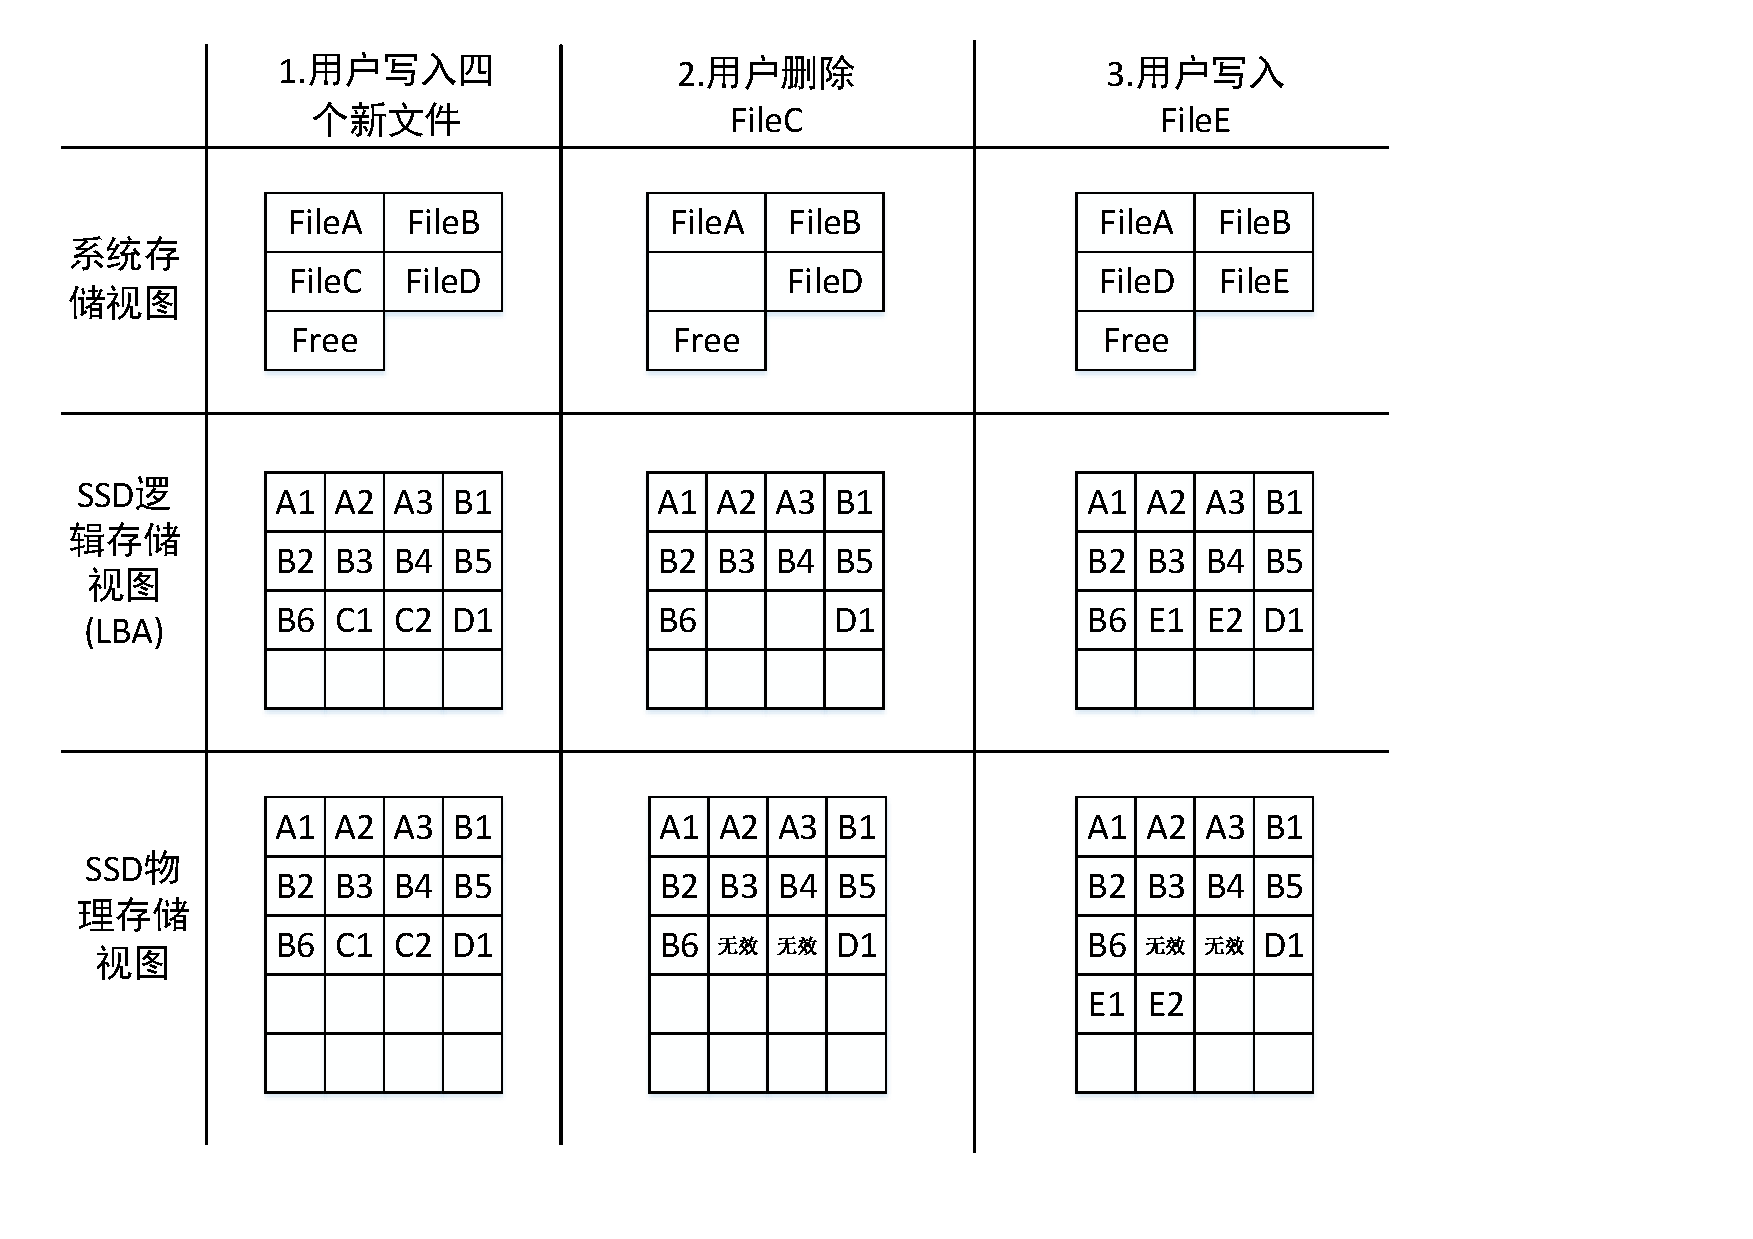
\includegraphics[width=4in]{Pics/trim.pdf}
	\caption{支持TRIM的固态盘删除、更新数据操作}\label{fig:2}
\end{figure}
在\autoref{fig:2}中的更新文件过程中,删除文件C时,删除指令立即调用內建的TRIM命令准备回收文件C占用的C1,C2两个数据块,物理介质上,这两个数据块已经被标记被“回收”状态,这样每次GC的时候就不用再移动C1、C2两个数据块,减少了数据泄露窗口和数据写入量。


如何确保原始数据不被非法地逆向解密读取出来,涉及到这套方案的冗余加密模块的两个关键参数:(1)直接参与运算的密钥数据;(2)加密后相互独立的数据块单元。只要将这两个条件中任意一个的数据“真正”地破坏掉,原始数据就再也无法恢复。


安全删除密钥数据,需要从物理意义上真正地将密钥擦除。目前,针对固态盘数据主流的物理擦除方法主要有以下三种:
\begin{itemize}
	\item 使用固态盘驱动器的ATA安全擦除。SSD固件有一个嵌入命令,可以将驱动器的每一个数据位覆写为0,从而达到安全删除数据的目的。这种擦除手段使用引导环境下的USB闪存盘,运行相应的清除工具即可以进行。
	\item 使用自加密驱动器的加密擦除。在一个自加密的固态盘驱动器(SED)上,加密密钥存储在驱动器的一块小型存储区域,由内部硬件加密待存储的数据和解密预备读取的数据,并且使用安全管理软件管理。我们可以将文件的加密密钥放置在该类SSD上,需要删除数据时。进入SED的管理软件,删除并重新生成固态盘的密钥。这将导致先前写入的密钥数据完全不可读。因此,冗余加密算法生成的数据也就无法还原成原始数据。
	\item 损坏密钥存储区的物理介质、这种擦除手段是将SSD介质通过标准的高温或者细化手段破坏,以至于不可再读。适用于安全要求非常高的应用场合。
\end{itemize}


为了适应大多数的固态盘的特性,本方案采用的是ATA安全擦除。一方面,带有自加密的固态盘厂商不一定完全设计实现,不能针对所有的固态盘硬件,并且物理或者化学方式的损坏不在本方案的讨论范围;另一方面,ATA安全擦除方法操作相对简单,而且即使系统被恶意破坏,我们也可以通过引导方式下的安全擦除(Secure Erase)功能擦除密钥,保证数据的安全性。


ATA安全擦除方法根据具体固态盘厂商的实现,內建的擦除命令使用的基本是覆写数据的方法,即对固态盘的物理页覆写特定的数据多次,达到无法恢复原始数据的目的,这种覆写手段通常最高能达到95.9-99.9\%的数据完全擦除\cite{Wei2011Reliably}。


在M.Wei的论文\cite{Wei2011Reliably}中指出,验证数据安全删除需要绕过文件系统,直接读取闪存芯片的数据。需要使用特殊的读取设备Ming the Merciless如\autoref{fig:3}所示。直接连接闪存芯片的针脚,读取其中的数据,从而避免了闪存转换层(FTL)的干扰。
\begin{figure}[H]
	\centering
	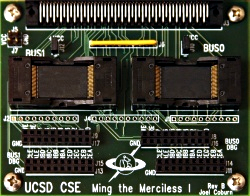
\includegraphics[width=2in]{Pics/ming.png}
	\caption{直接读取闪存芯片设备}
    \label{fig:3}
\end{figure}
针对本方案涉及到的两个关键问题:(1)数据安全删除;(2)系统可用性或者是可靠性。技术关键就是为了解决怎样安全删除的问题,系统可靠性应该依赖于在解决安全删除的基础之上进行的改进。
\section{系统详细设计}
\subsection{模块架构}
将多个SSD组成一个存储阵列。对于上层组件,如文件系统,将SSD看做一个简单的块设备,而不关心其内部的负载结构。用户可以在上面创建分区和文件系统,和普通硬盘一样。这样很容易整合到现有系统,因为对整个系统的改动很小。整体模块架构如\autoref{fig:4}所示。


其中,有一个单独的元数据盘用来存储系统初始化时产生的一段随机数据,和原始数据的哈希信息这些元数据,元数据的总量很小,但却是
整个系统在进行读取还原数据或者是安全删除时,这部分数据都是关键的信息。攻击者在无法获取这部分元数据时,是无法窃取到原始数据的。


用于存储元数据的固态盘容量也相应的非常小,比如一个16GB的闪存盘就可以存储这些数据。这样,安全删除数据时,
只要擦除元数据盘上的全部数据,就可以达到数据安全的目的。而且,针对小容量的固态盘的全盘删除,因为数据量小,
对固态盘的寿命影响也比较小。
\begin{figure}[H]
	\centering
	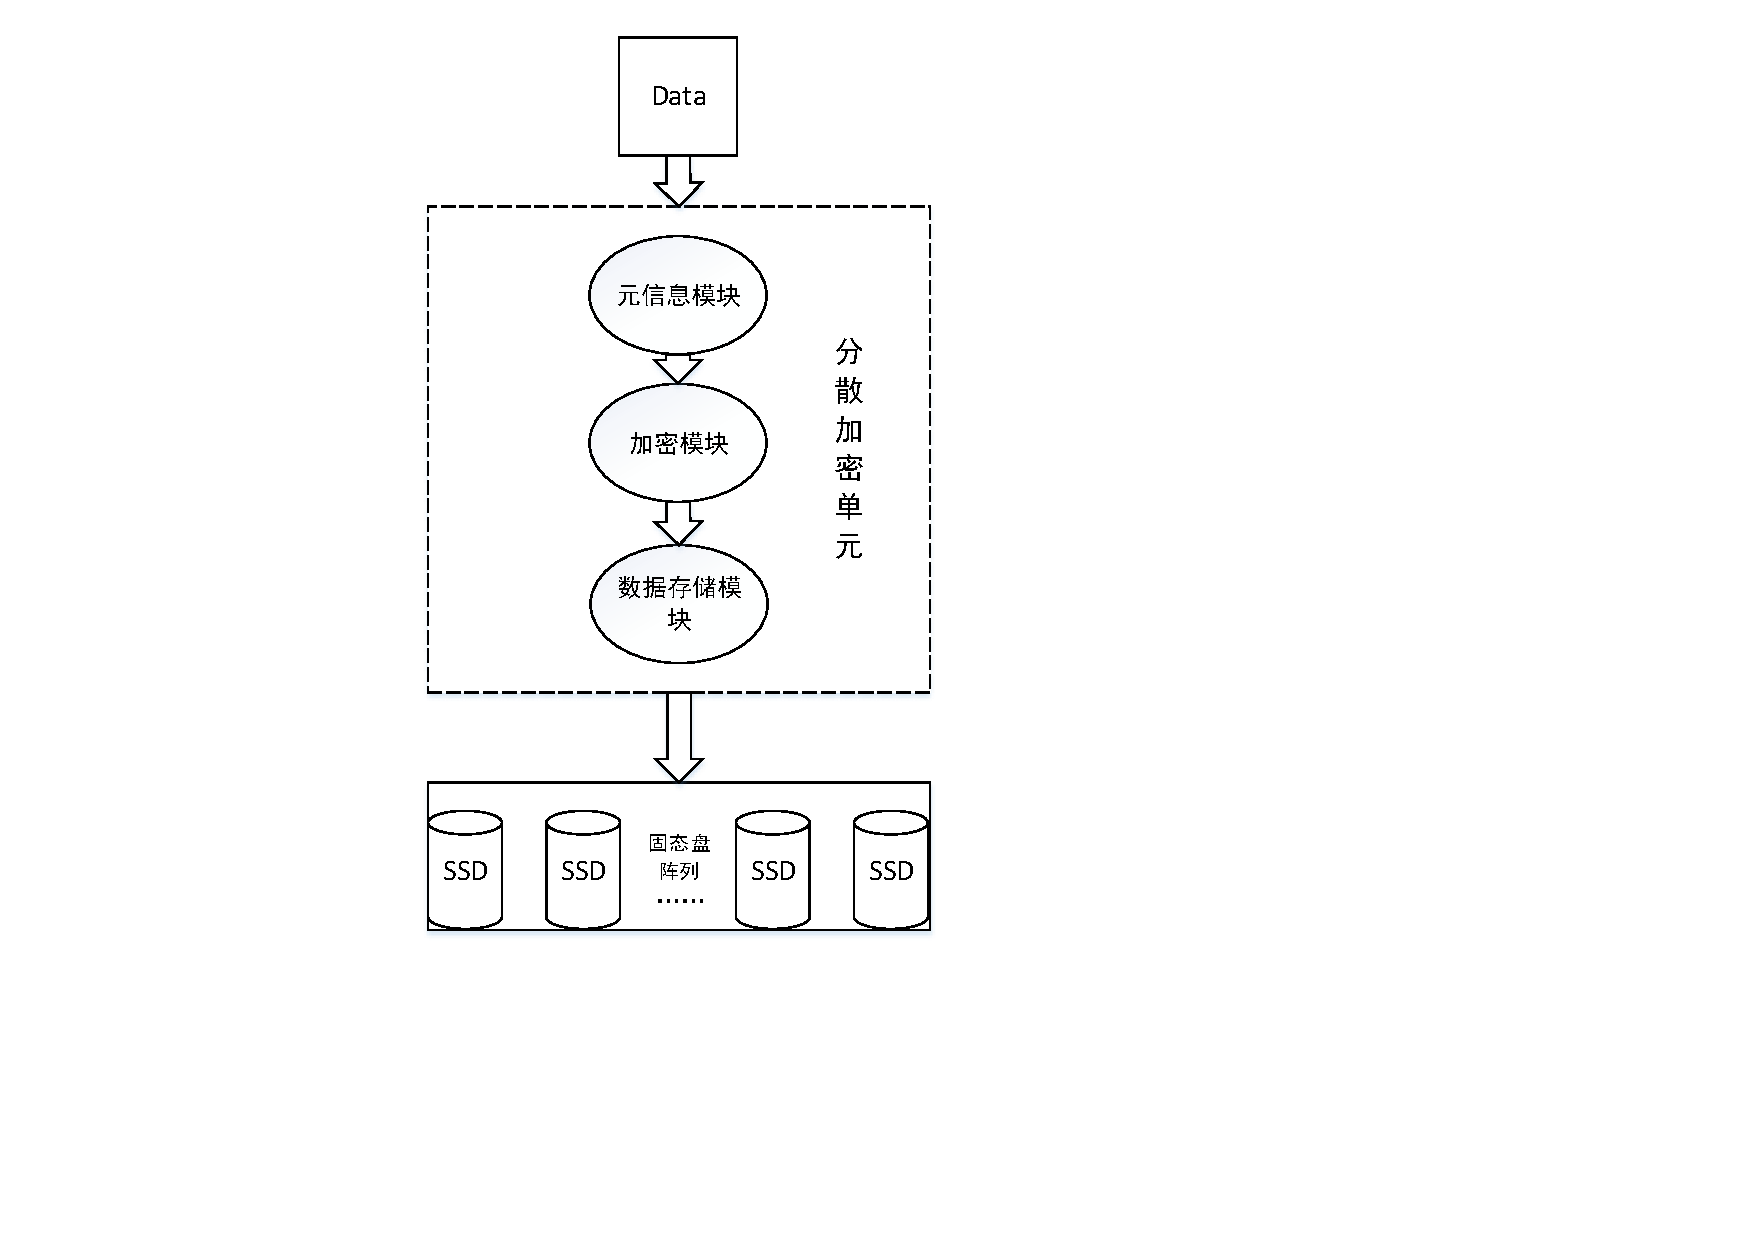
\includegraphics[width=3in]{Pics/total-structure.pdf}
    \caption{模块功能架构}
    \label{fig:4}
\end{figure}
原始数据经过分散加密系统,首先是数据分成一个个的加密单元数据块,在系统中目前选取的平均数据块大小是8k,然后由数据标记中心记录原始数据块的元数据,并将元数据与数据块进行多次的哈希和异或、非对称加密运算,得到初始加密数据块,最后通过冗余编码,得到编码数据块,将这些数据块写入阵列的相应独立区域中。
\subsection{编码原理}
纠删码是存储领域常用的数据冗余技术,相比多副本存储而言,纠删码能够以更小的数据冗余度获得更高的数据可靠性。本方案采用的是
Reed Soloman编码\cite{Plank1996A,Plank2013Erasure}。它的基本原理如下:给定n个数据块$d_1$,$d_2$,...,$d_n$,n和一个正整数m,RS根据n个数据块生成m个校验块$c_1$,$c_2$,...,$c_m$。对于任意的n和m,从n个原始数据块和m个校验块中任取n块就能解码出原始数据。


RS编码最多容忍m个数据块或者校验块同时丢失。当存储的数据单元丢失或者被破坏到大于m个数据单元时,原始数据将无法被恢复,从而保证了数据的安全。具体的RS编码步骤如\autoref{fig:encode}所示。
\begin{figure}[H]
	\centering
	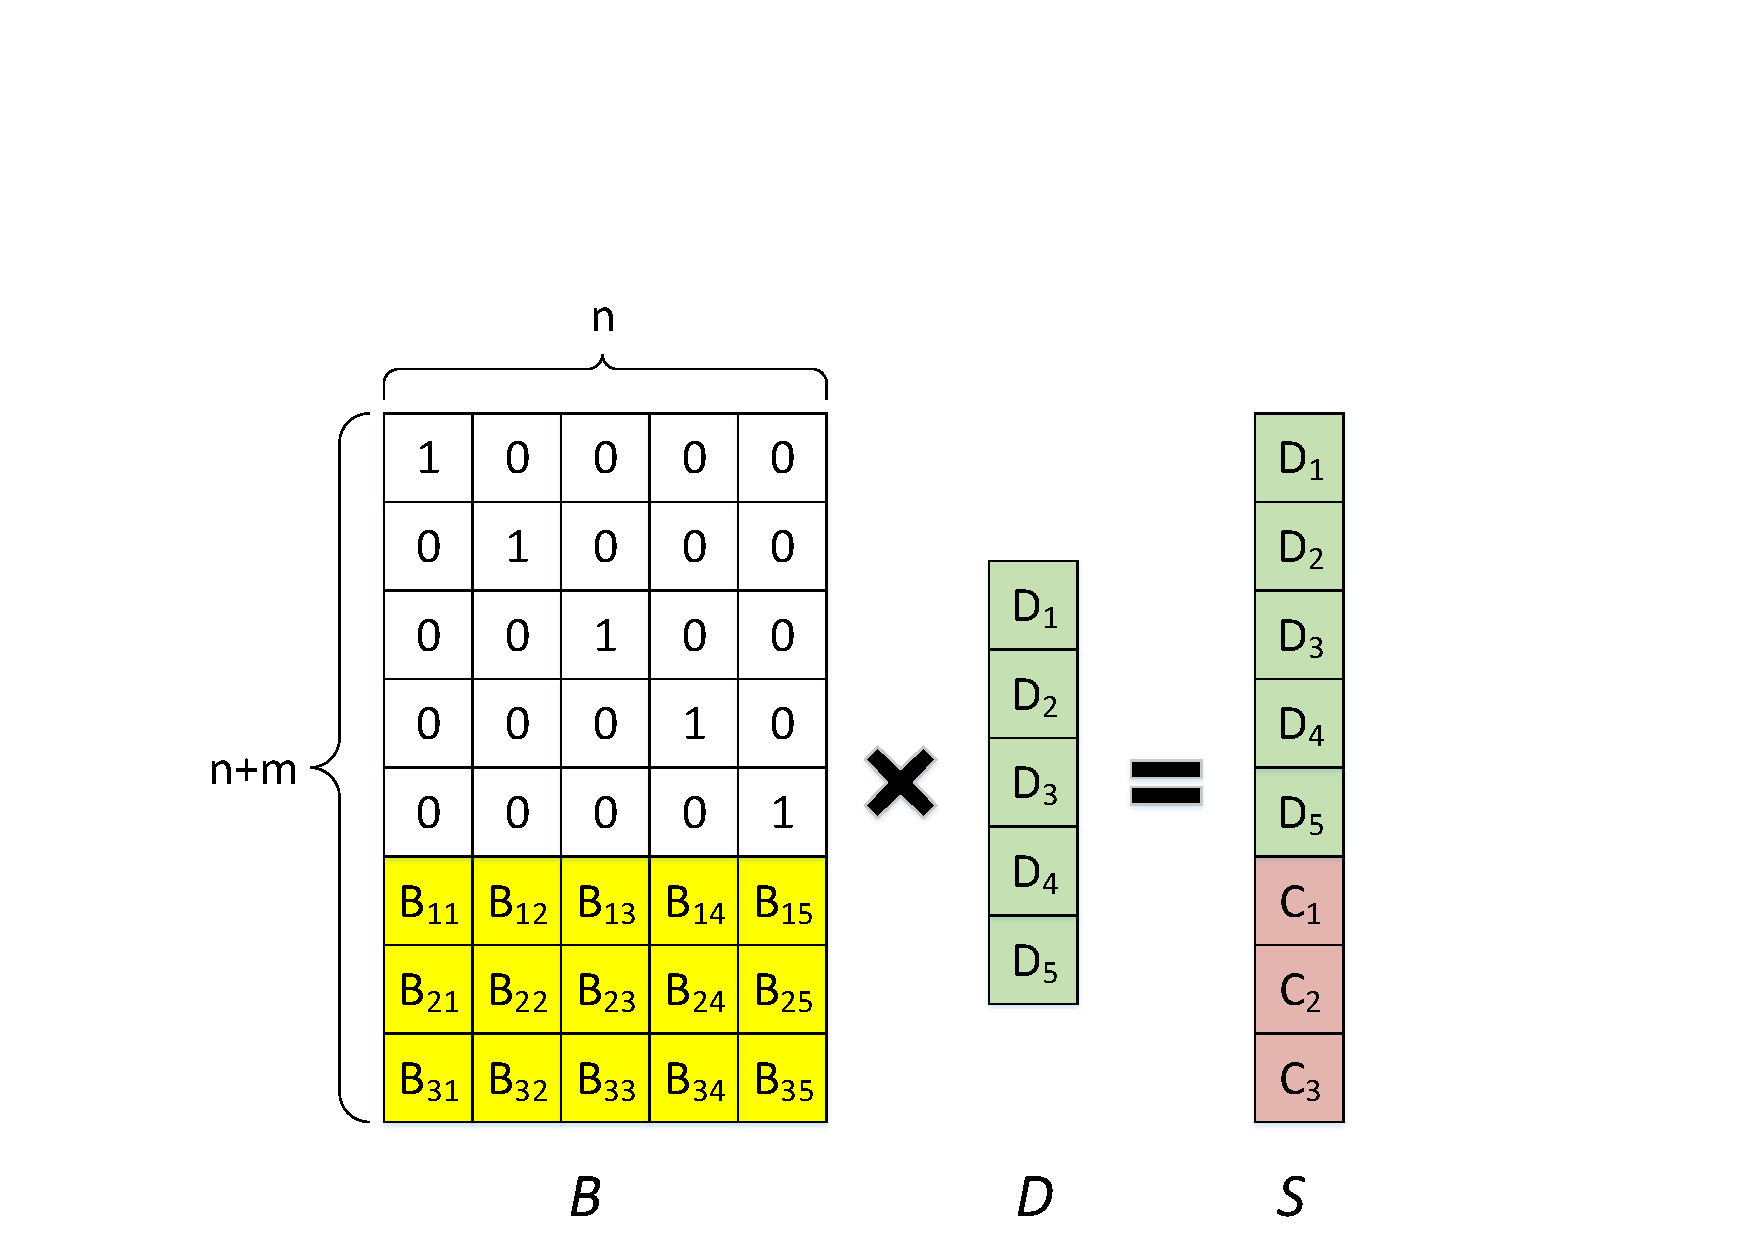
\includegraphics[width=4in]{Pics/encode.pdf}
	\caption{编码运算}\label{fig:encode}
\end{figure}
输入数据视为向量D={$D_1$,$D_2$,...,$D_n$},编码后数据视为向量S={$D_1$,$D_2$,...,$D_n$,$C_1$,$C_2$,...,$C_m$}。图\autoref{fig:encode}左边是编码矩阵,矩阵上部是单位矩阵(n行n列),下边是vandermonde矩阵矩阵B(m行m列),vandermonde矩阵如图\autoref{fig:vandermonde}所示。第i行第j列的元素值为$j^(i-1)$。
\begin{figure}[H]
	\centering
	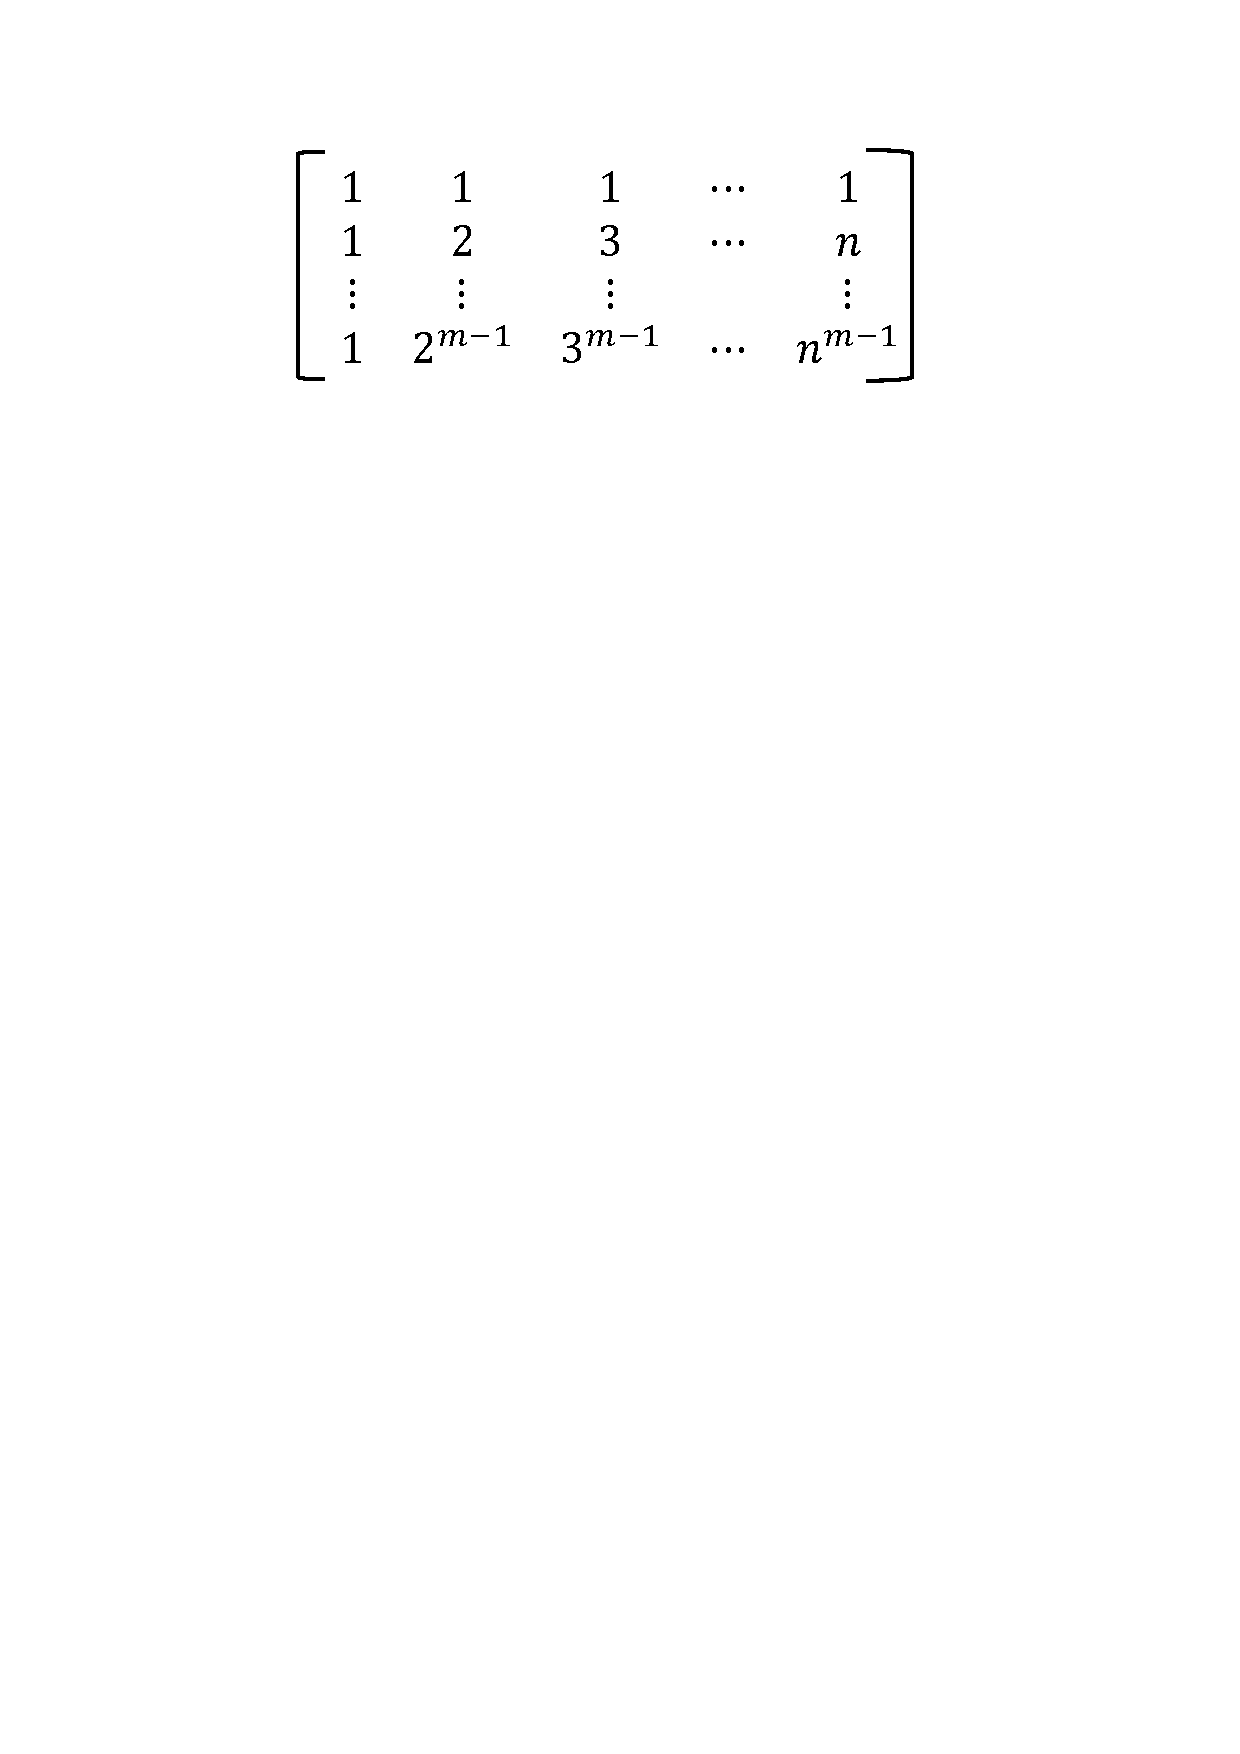
\includegraphics[width=3in]{Pics/vandermonde.pdf}
	\caption{vandermonde矩阵}\label{fig:vandermonde}
\end{figure}
因为RS数据恢复算法要求编码矩阵的任意n*n子矩阵可逆,所以这里采用了vandermonde矩阵。
数据D经过编码后得到了数据S,其中包含原始的数据S和校验数据C,这就是我们最终存储的加密数据单元。


\subsection{冗余加密算法}
数据编码算法主要借鉴了M.Li\cite{Li2014Convergent}的冗余加密思想,将数据和元数据,以及系统随机的一段初始化数据混合
在一起经过多次的非对称加密、冗余编码得到最终的加密数据单元。这种算法在删除了元数据这些关键数据后,原始数据将无法
恢复。整体加密流程如\autoref{fig:5}所示。
\begin{figure}[H]
	\centering
	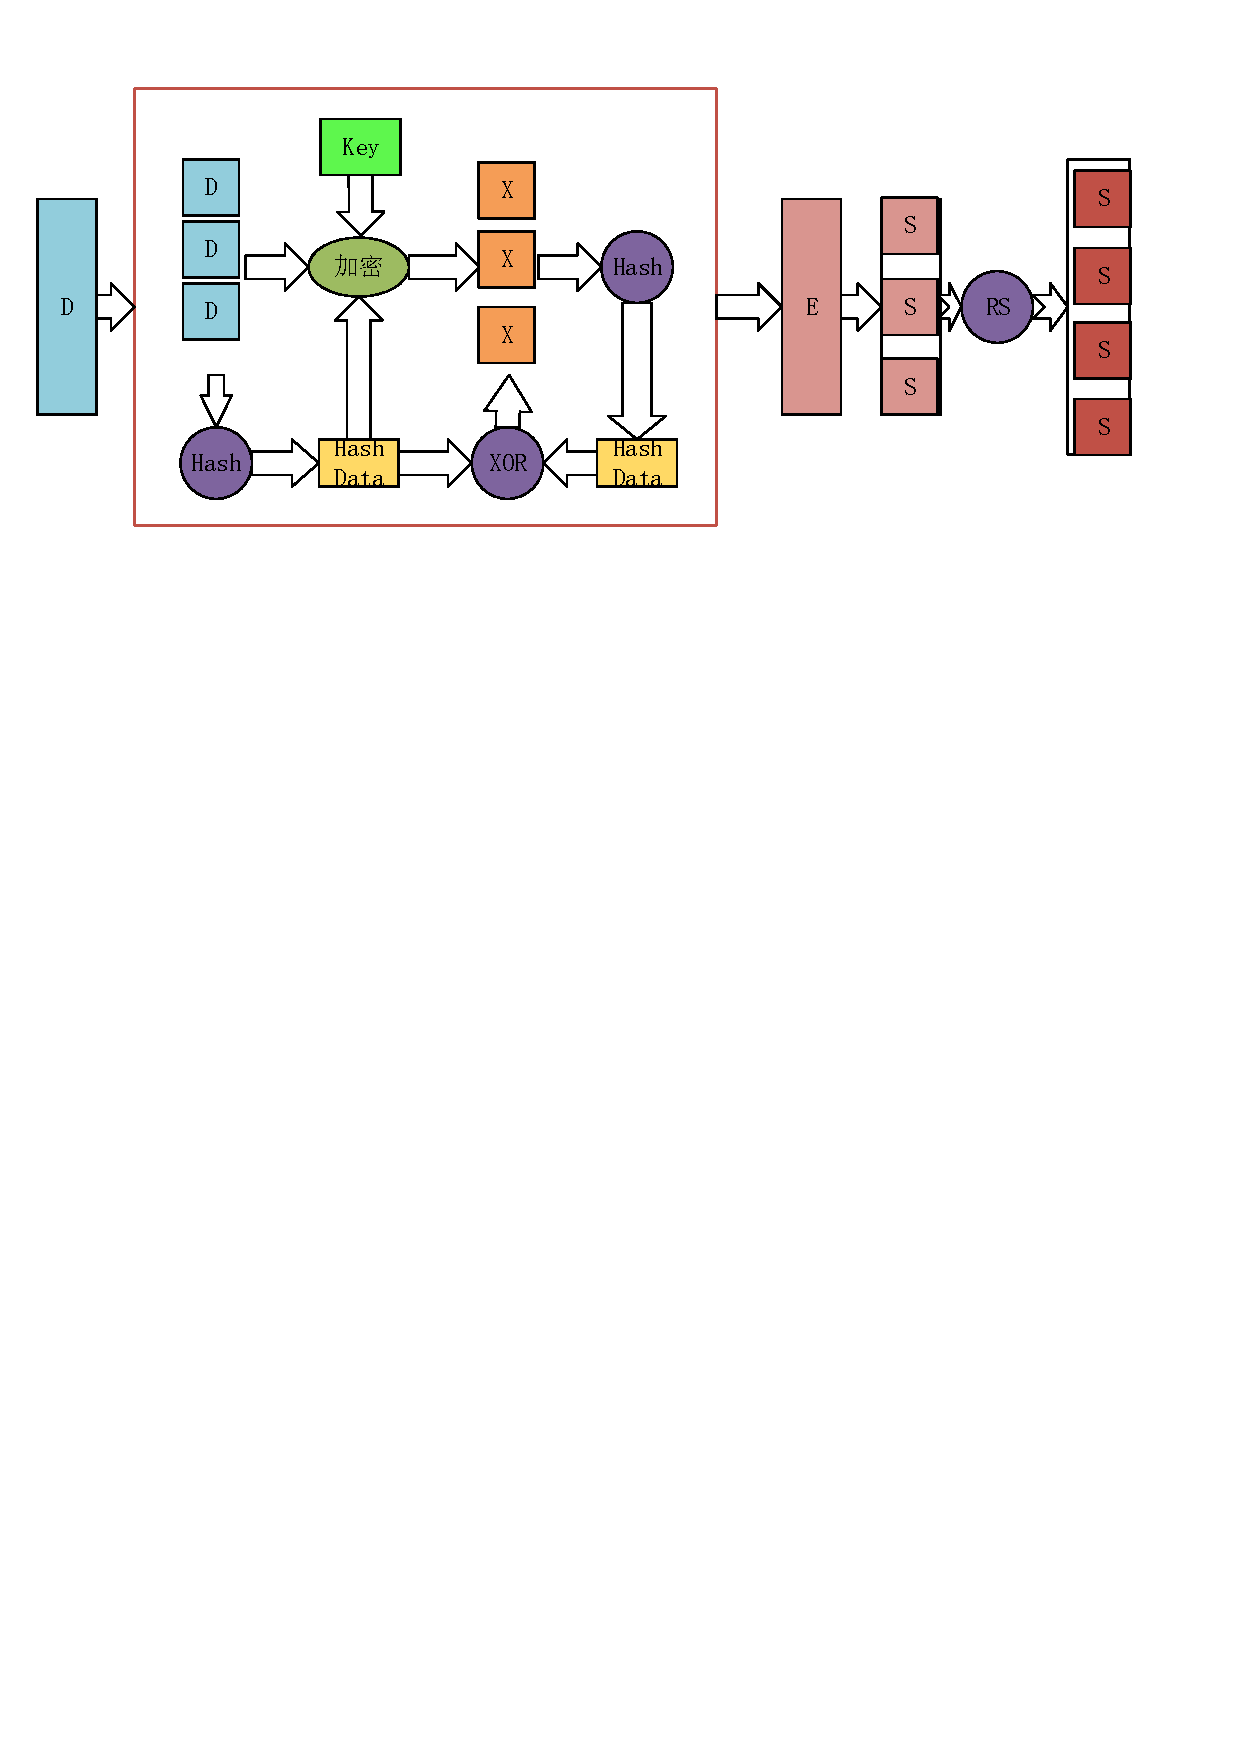
\includegraphics[width=4in]{Pics/encrypt.pdf}
	\caption{加密算法流程}\label{fig:5}
\end{figure}
加密模块在输入原始数据块后,首先分为大小一定的数据块,进行一系列的哈希运算和加密操作后,得到初始的加密数据块X,再由X的哈希信息数据和之前原始数据的哈希信息数据异或操作得到初步的加密数据块。这些数据块组合成大小相同的加密数据单元S,最后由冗余运算模块操作得到最终的加密存储数据。详细的加密流程与算法如\autoref{eq:1}所示。
\begin{equation}
    \label{eq:1}
    \begin{aligned}
        c_{i} &=d_{0} \bigoplus E(h_{key},i),i=0,1,...,s-1 \\ % 注释有特殊符号
        c_{s} &=h_{key} \bigoplus H(c_0,c_1,...,c_{s-1})     
    \end{aligned}
\end{equation}
\footnote{$\bigoplus$ 表示异或操作
\newline h$_{key}$表示对数据块取哈希操作,安全领域使用的主流哈希算法有SHA-1、SHA-256等
\newline E表示非对称加密算法,常用的算法有AES-128、AES-256
}

\begin{enumerate}
    \item 将原始数据D分割成d$_{0}$,d$_{1}$,...,d$_{s-1}$共s个数据块,按照\autoref{eq:1}的运算得到初步加密后的数据块c$_{1}$ ,c$_{2}$,…,c$_{s}$
	\item 加密后的数据块经过群运算得到最终相互独立的加密数据单元
\end{enumerate}

\subsection{数据恢复原理}
在数据被多次加密运算,并且经过RS编码后,得到了最终的冗余加密数据。在编码原原理一节中提到,RS最多容忍m个数据丢失,当有m个数据没有参与解码运算时,数据恢复过程如下。


1.从编码矩阵B中删除丢失数据块和丢失编码块对应行。假设$D_1$,$C_2$丢失,根据图\autoref{fig:encode}所示的RS编码运算等式,我们得到新的编码矩阵$B^{'}$以及等式如图\autoref{fig:decode}所示。
\begin{figure}[H]
	\centering
	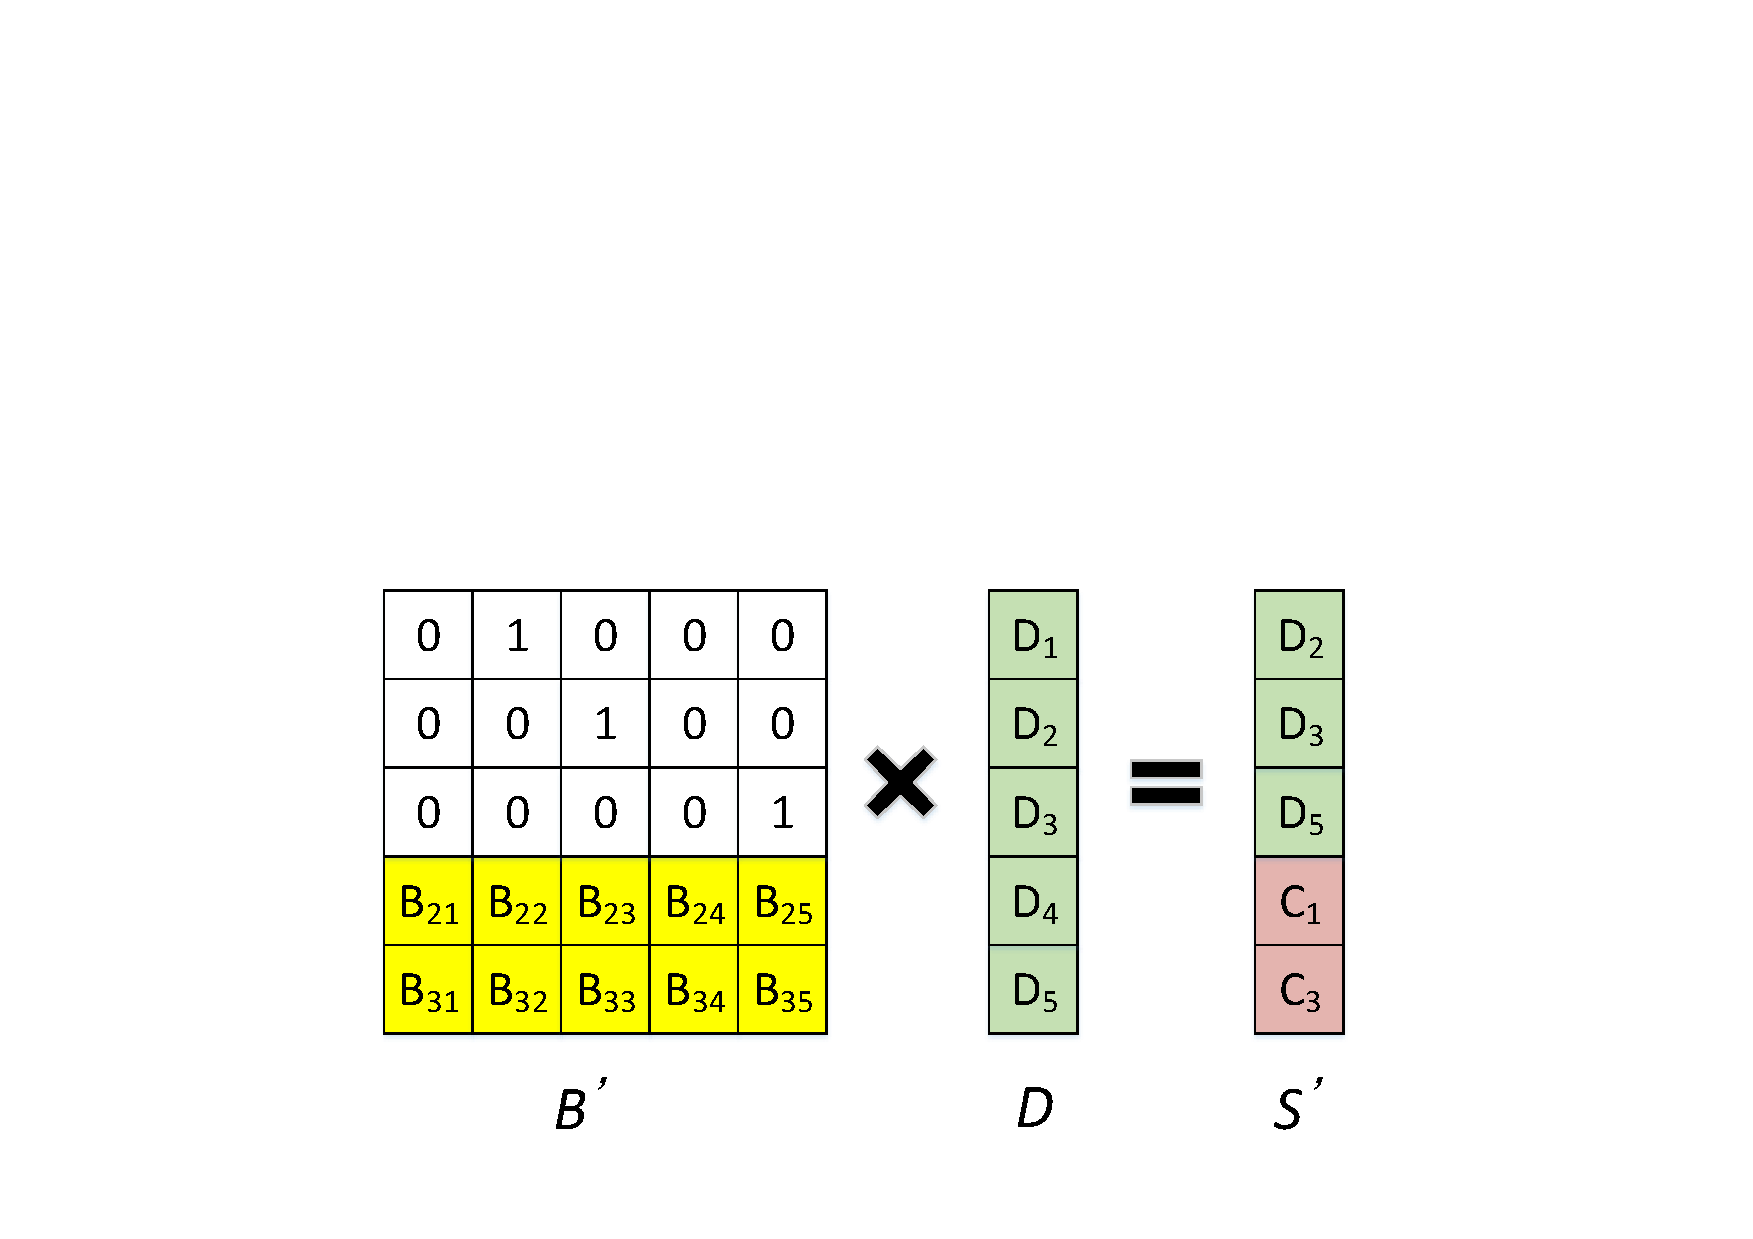
\includegraphics[width=4in]{Pics/decode.pdf}
	\caption{新编码矩阵运算式}\label{fig:decode}
\end{figure}


2.由于$B^{'}$是可逆的,等式两边乘上$B^{'}$的逆矩阵$B^{'-1}$,得到如下等式\author{fig:decode2}。
\begin{figure}[H]
	\centering
	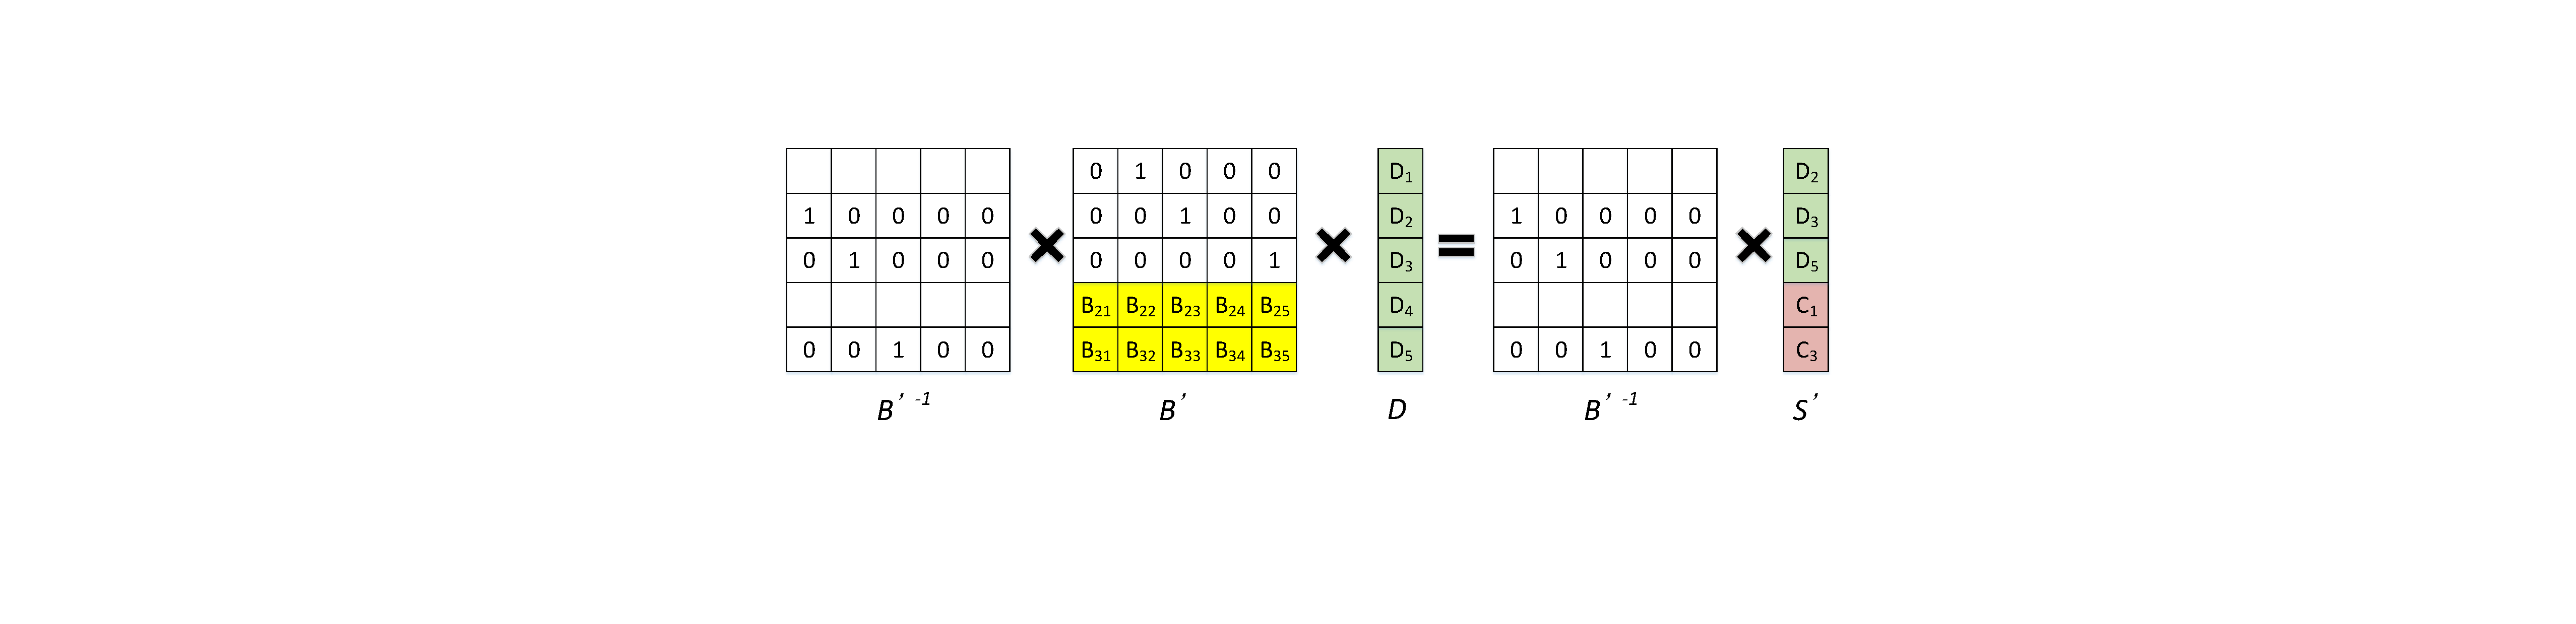
\includegraphics[width=4in]{Pics/decode2.pdf}
	\caption{同乘$B^{'-1}$矩阵运算式}\label{fig:decode2}
\end{figure}


3.将等式\autoref{fig:decode2}化简,就得到了原始数据D的恢复算法公式\autoref{fig:decode3}。
\begin{figure}[H]
	\centering
	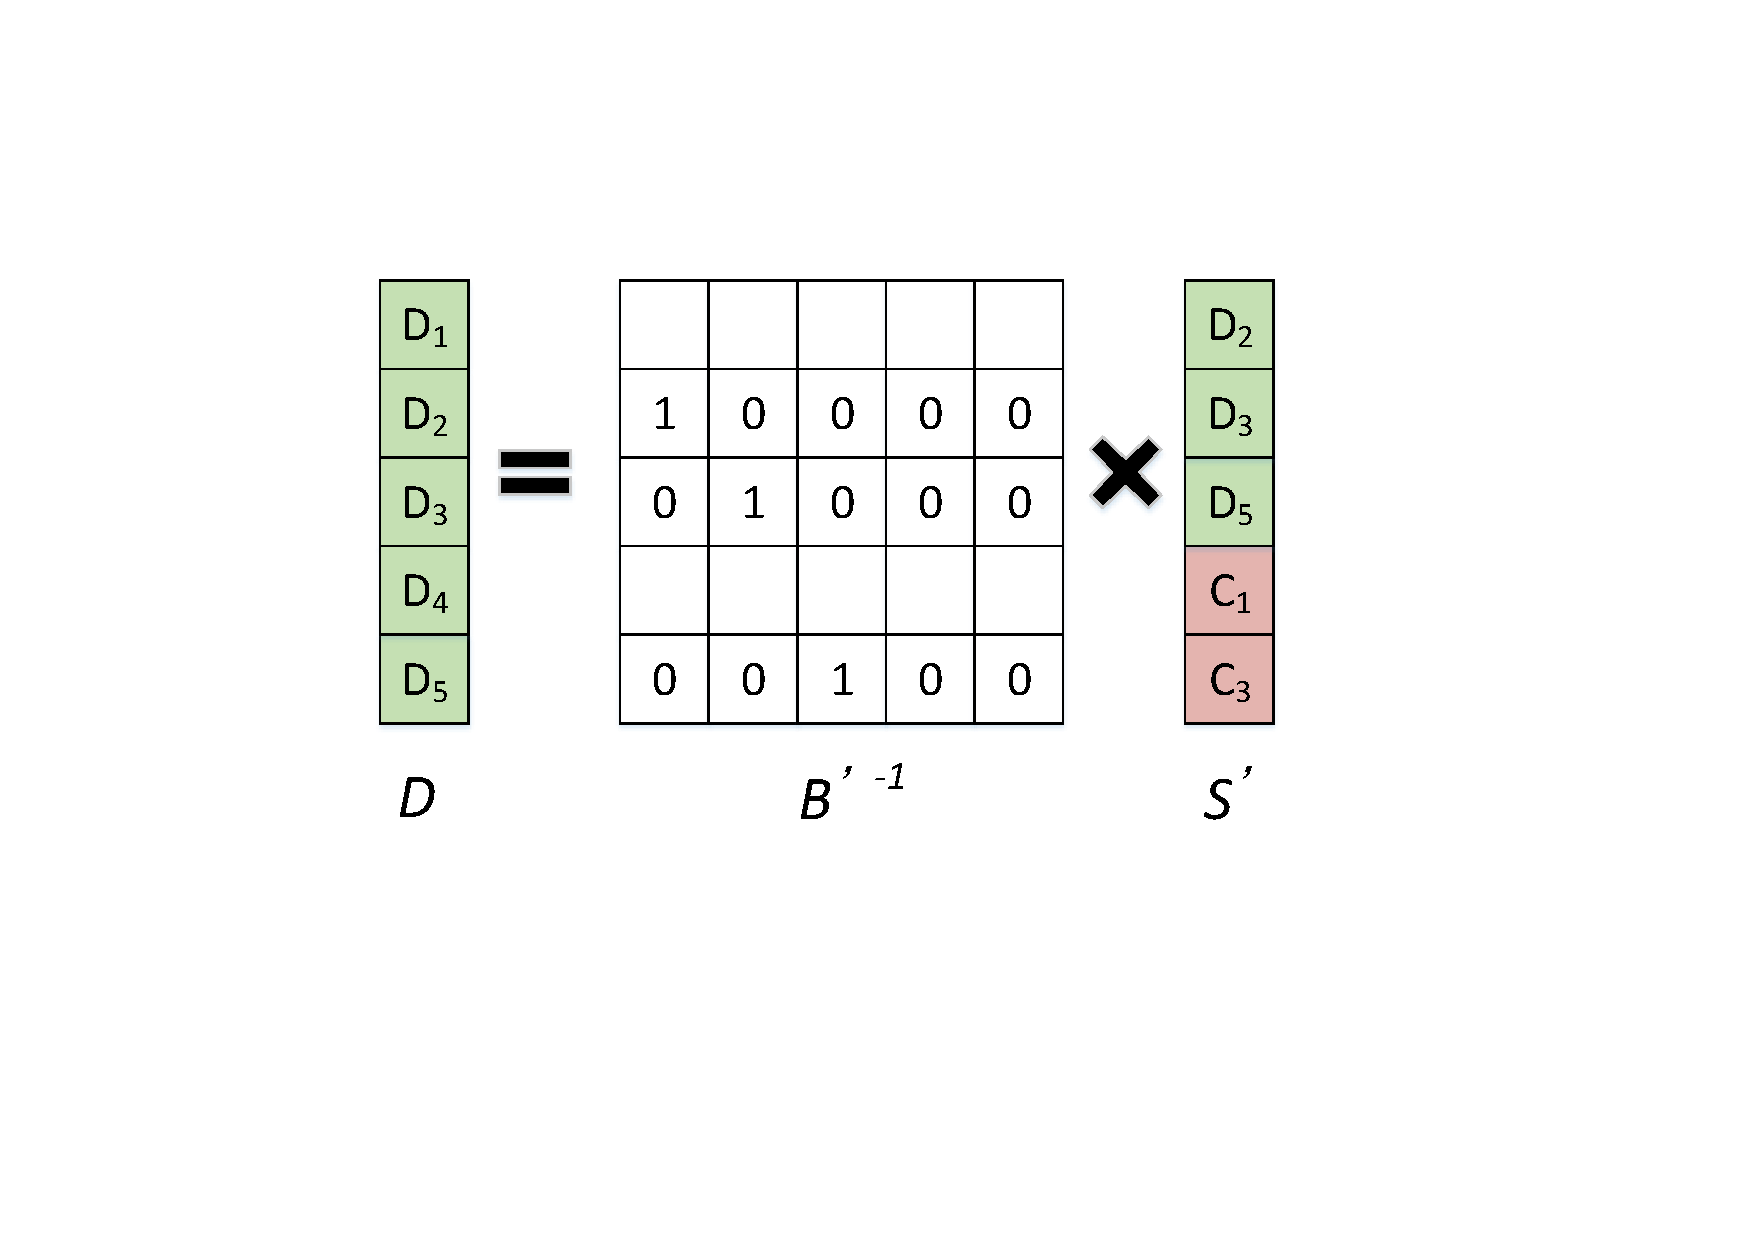
\includegraphics[width=4in]{Pics/decode3.pdf}
	\caption{RS恢复数据编码}\label{fig:decode3}
\end{figure}


4.对D重新编码,得到丢失的校验数据块$C_2$,至此所有的数据均被恢复。


在矩阵求逆的过程中,使用的高斯消元法无法作用于定字长w的二进制数据。RS编码采用伽罗瓦群GF($2^w$)中定义的四则运算法则,GF($2^w$)域有$2^w$个值,每个值都对应一个低于w次的多项式,通过这种方式,域上的四则运算转化成多项式空间的运算。GF($2^w$)域中的加法就是异或XOR操作,
乘法需要维护两个大小为2$^{w}-1$的表格:log表gflog和反log表gfilog。乘法公式如公式\autoref{eq:multiply}所示。
\begin{equation}
\label{eq:multiply}
\begin{aligned}
    a * b &=gfilog(gflog(a) + gflog(b)) \% (2^w-1)
\end{aligned}
\end{equation}

\subsection{破坏恢复条件}
前面已经提到,为了使原始数据再不可恢复,针对加密后的数据,可以有两种解决办法:一是至少删除n-r份数据单元的加密数据,使得RS解码数据块的条件被破坏;二是完全删除元数据,没有元数据参与解密运算,此时就无法解密出原始数据。两种删除方法分别对应\autoref{fig:6}和\autoref{fig:7}所示。
\begin{figure}[H]
	\centering
	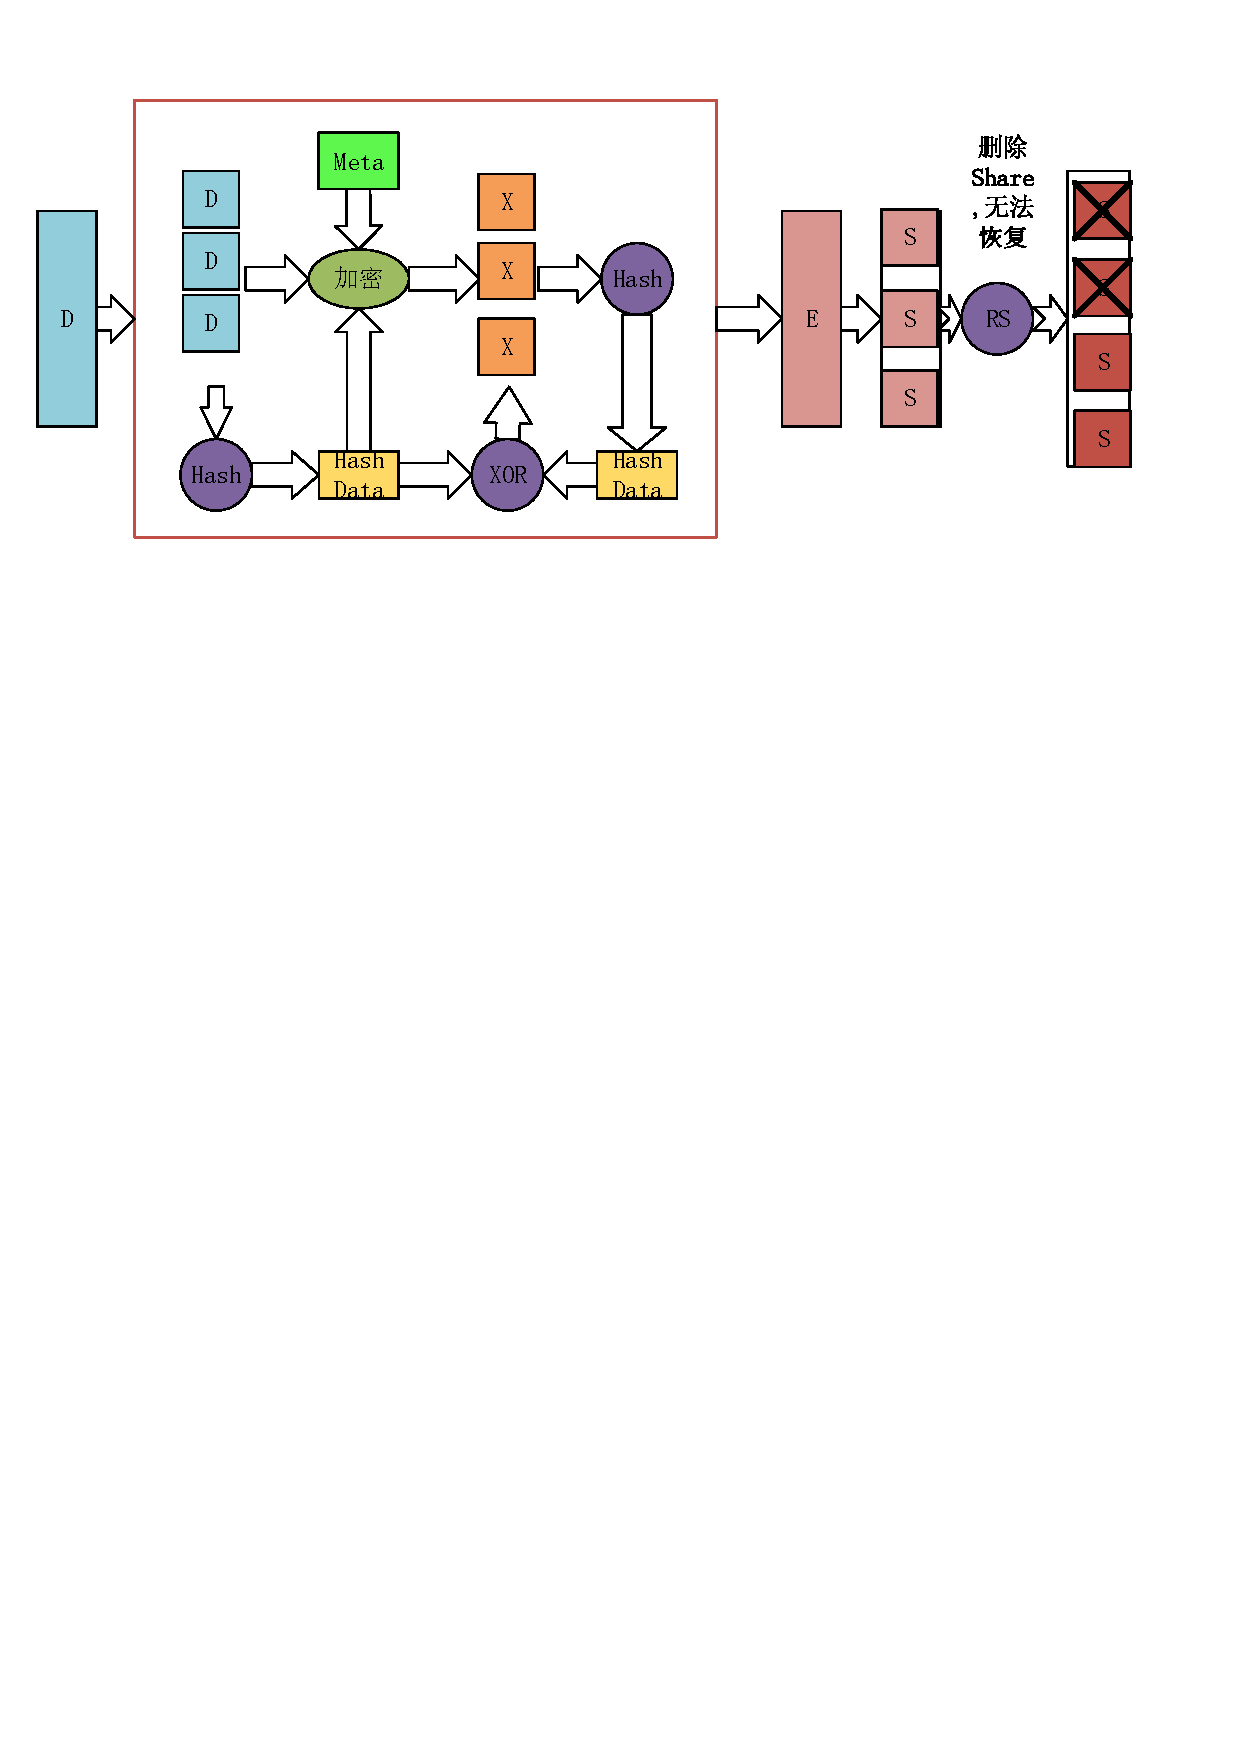
\includegraphics[width=4in]{Pics/del-share.pdf}
	\caption{删除数据块的方法}\label{fig:6}
\end{figure}
\begin{figure}[H]
	\centering
	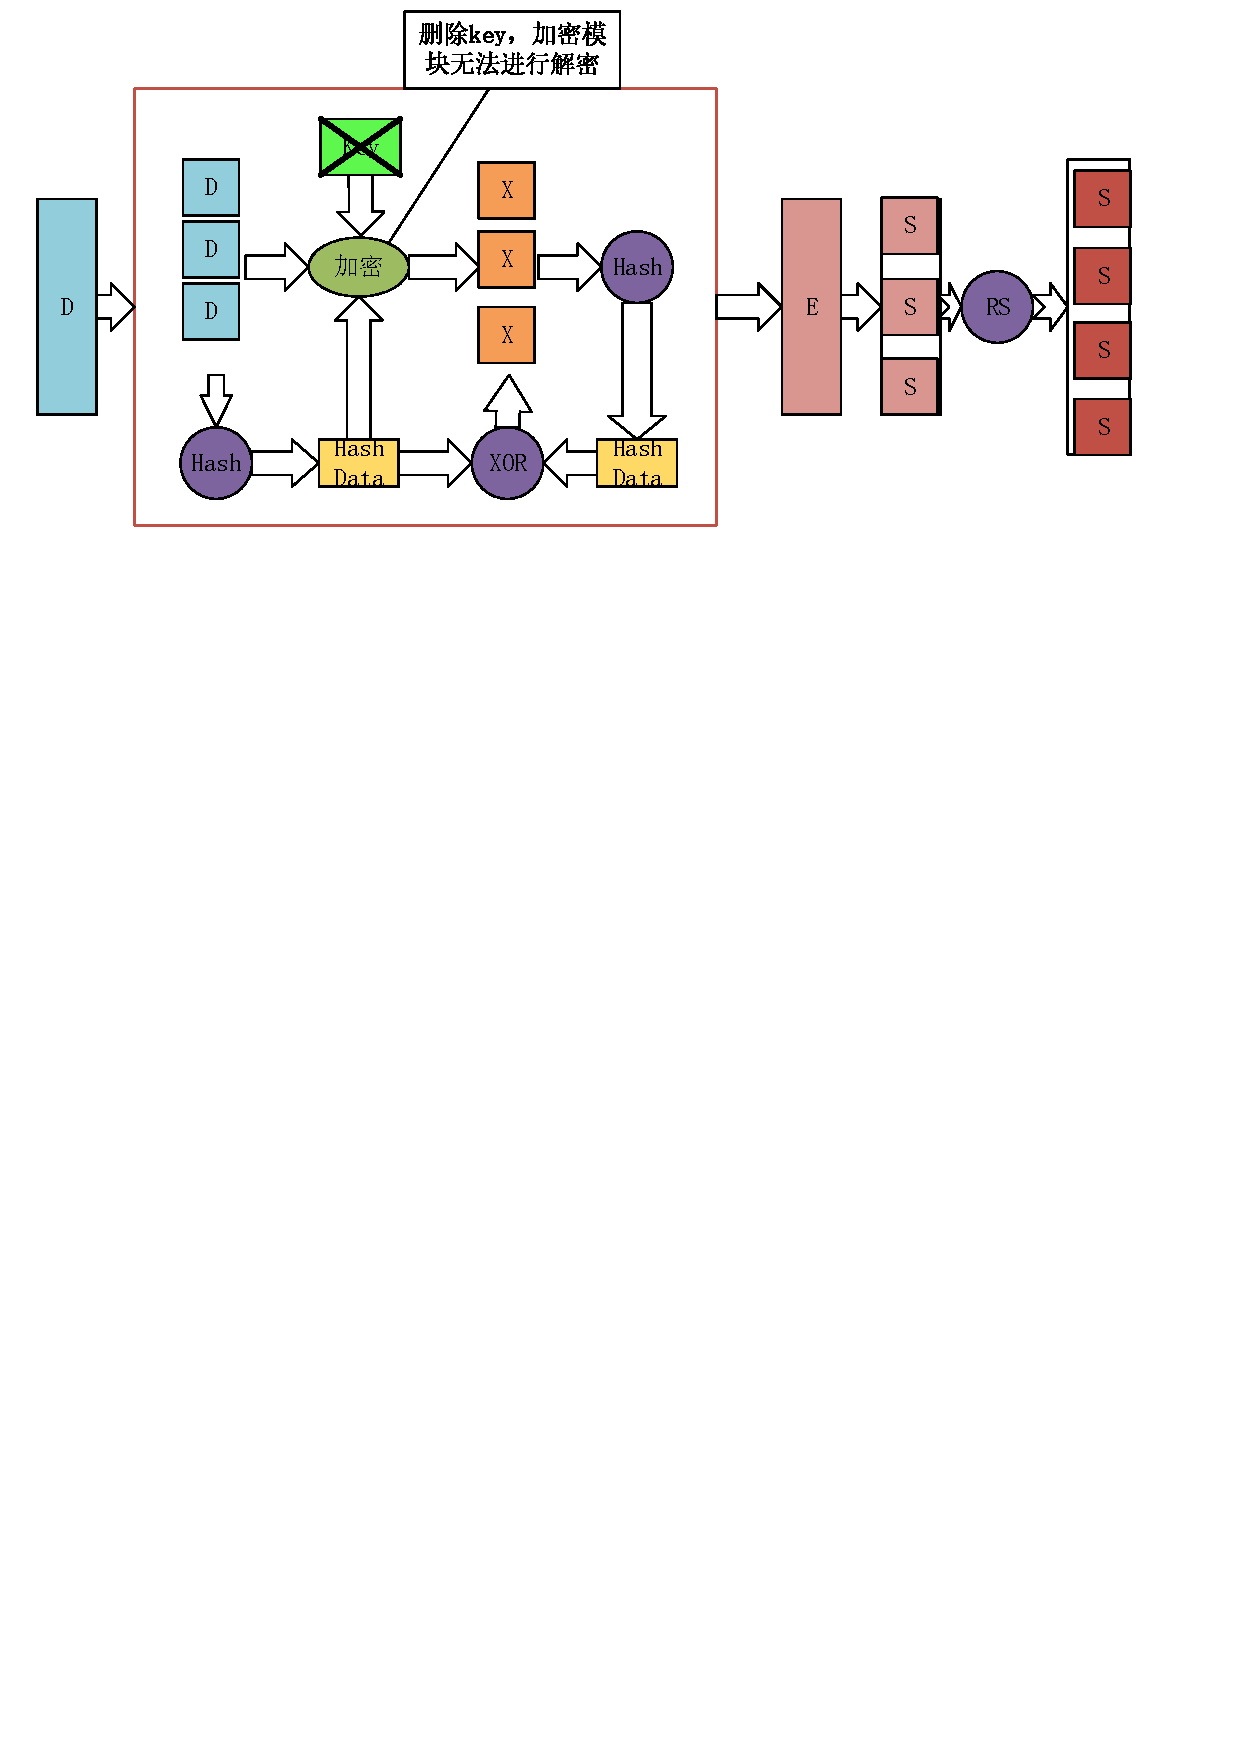
\includegraphics[width=4in]{Pics/del-hashkey.pdf}
	\caption{删除存储的元数据}\label{fig:7}
\end{figure}


这里我们选择的是删除原始文件的元数据,有如下三个原因:
\begin{itemize}
	\item 元数据通常都比较少,而且大小固定。可以利用固态盘的特殊性,安全的删除。而删除Share数据量太大,对固态盘阵列来说,势必会降低其使用寿命。
	\item 固态盘使用TRIM指令可以很快速地完全删除,真正地达到清除存储数据的地步。而完全删除相互独立的加密数据单元是一件非常耗时的操作,会显著影响系统的可用性,在一些频繁更新和删除文件的场合,这种方案的劣势会更加突出。
	\item 可以将文件及相关的元数据存放在一个独立的固态盘上,需要删除时,直接使用擦除软件安全删除密钥,管理比较方便。而删除加密数据单元的手段比较费时费力,无法集中管理。
\end{itemize}

\subsection{从物理介质上删除敏感信息数据}
本方案采用的是将哈希信息等元数据单独存储在一个固态盘上,需要删除对应的数据时。使用ATA低级擦除方法擦除该固态盘数据,即多次写入方法,首先数据位全部覆写0,然后写入随机数据,最后再次写入0数据,达到安全删除的效果\cite{Lee2008Secure,Swanson2010Safe}。
%目前,使用经过验证的Parted Magic这类软件的安全擦除法,能够确实有效地物理擦除数据。
\section{系统整体流程}
本文采用的方案是在SSD组成的混合存储结构上,分出一个单独的密钥盘存放密钥数据,使用多个SSD组成盘阵,用来存放加密后的数据单元。整体结构如\autoref{fig:8}所示。
\begin{figure}[H]
	\centering
	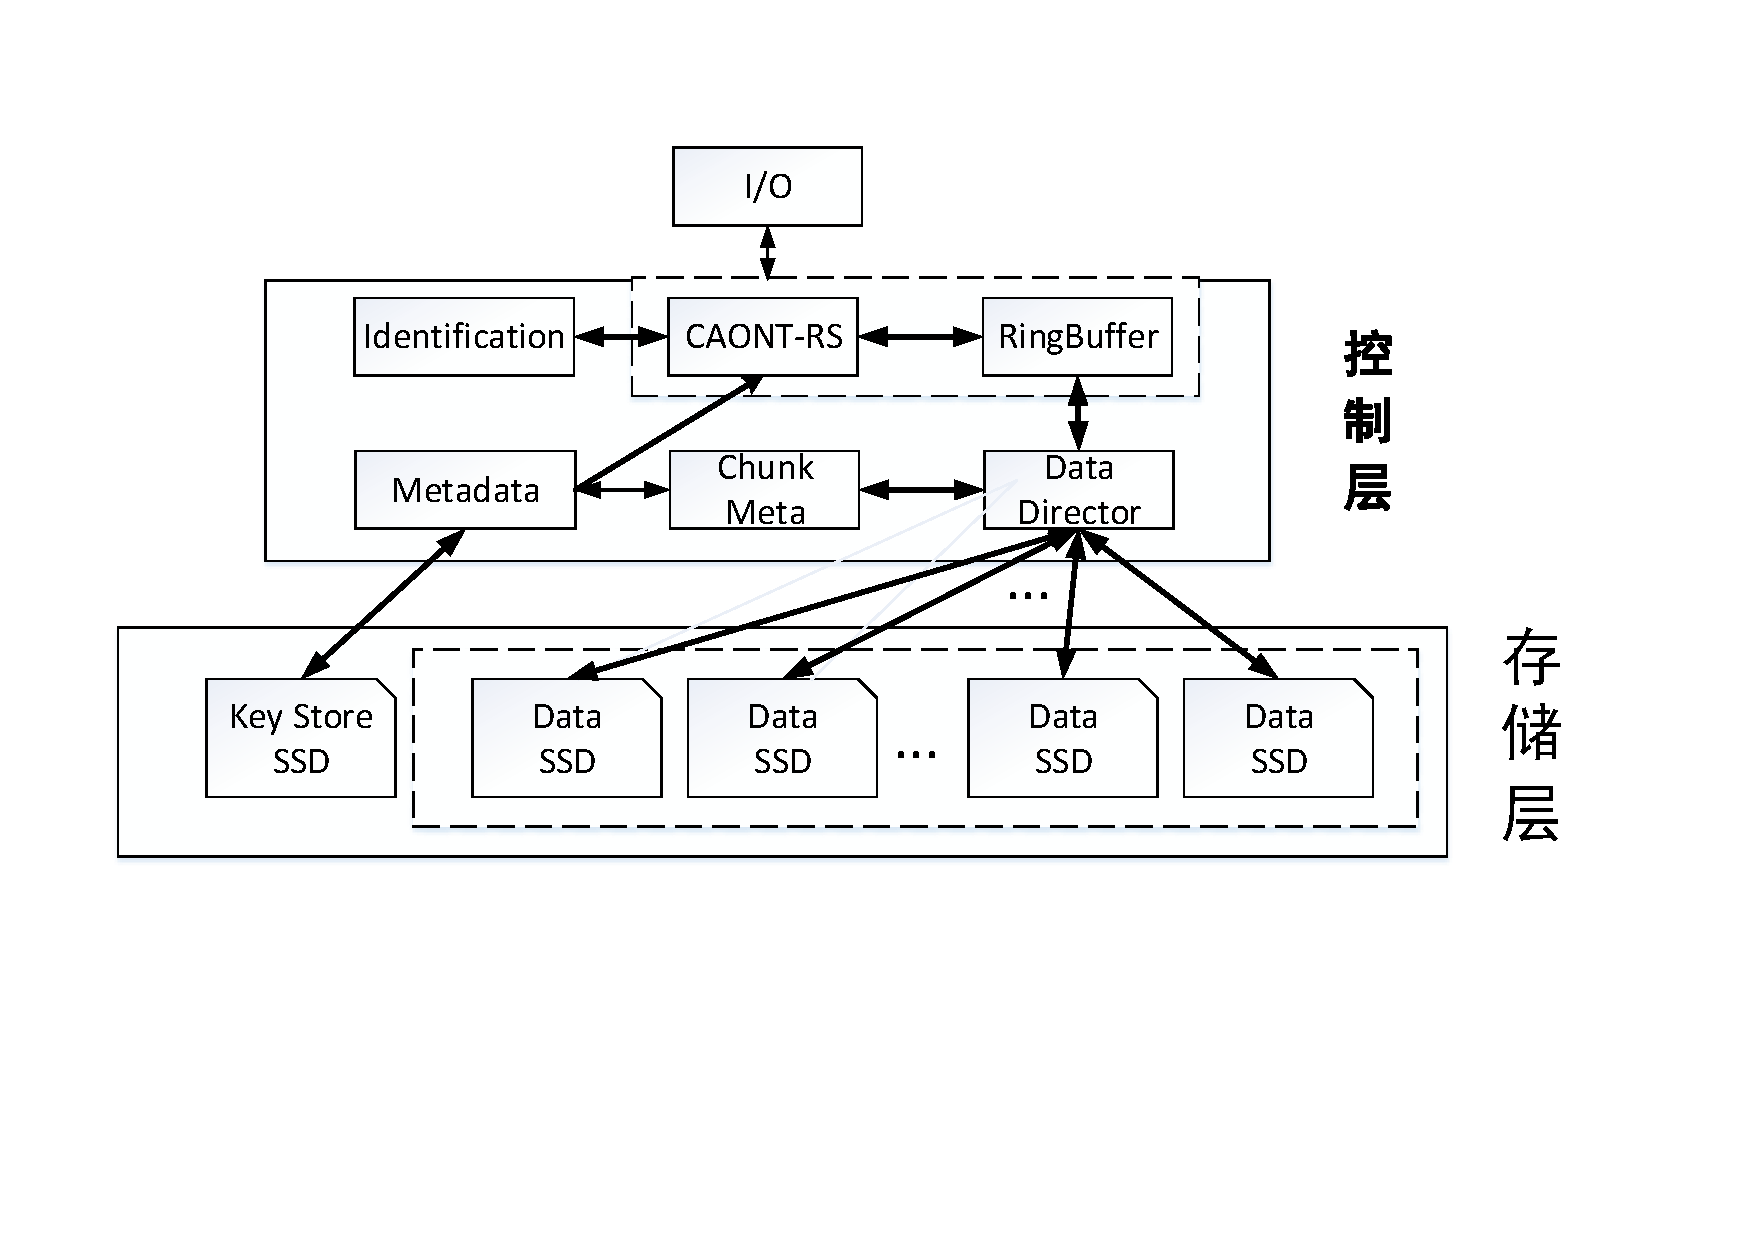
\includegraphics[width=1\textwidth]{Pics/total-store-structure.pdf}
	\caption{系统整体架构}\label{fig:8}
\end{figure}
当有I/O请求到来时,逻辑控制层首先将数据分成固定大小的数据块,标记每一个数据块的序号。同时,一段随机32位数据与数据块的元数据输入冗余加密模块进行加密和冗余编码,生成冗余数据块,输出到循环队列中缓存等待存储。文件信息管理模块记录下加密后的数据块的编号,由数据分发模块将相互独立的数据单元有序分发到数据盘。与此同时,元数据存储在密钥盘。在安全删除部分,我们只需要将密钥盘安全擦除数据即可。\\
下面结合本方案的具体功能详细描述系统读、写、删除的流程。
\subsection{系统写入数据}
\begin{figure}[H]
	\centering
	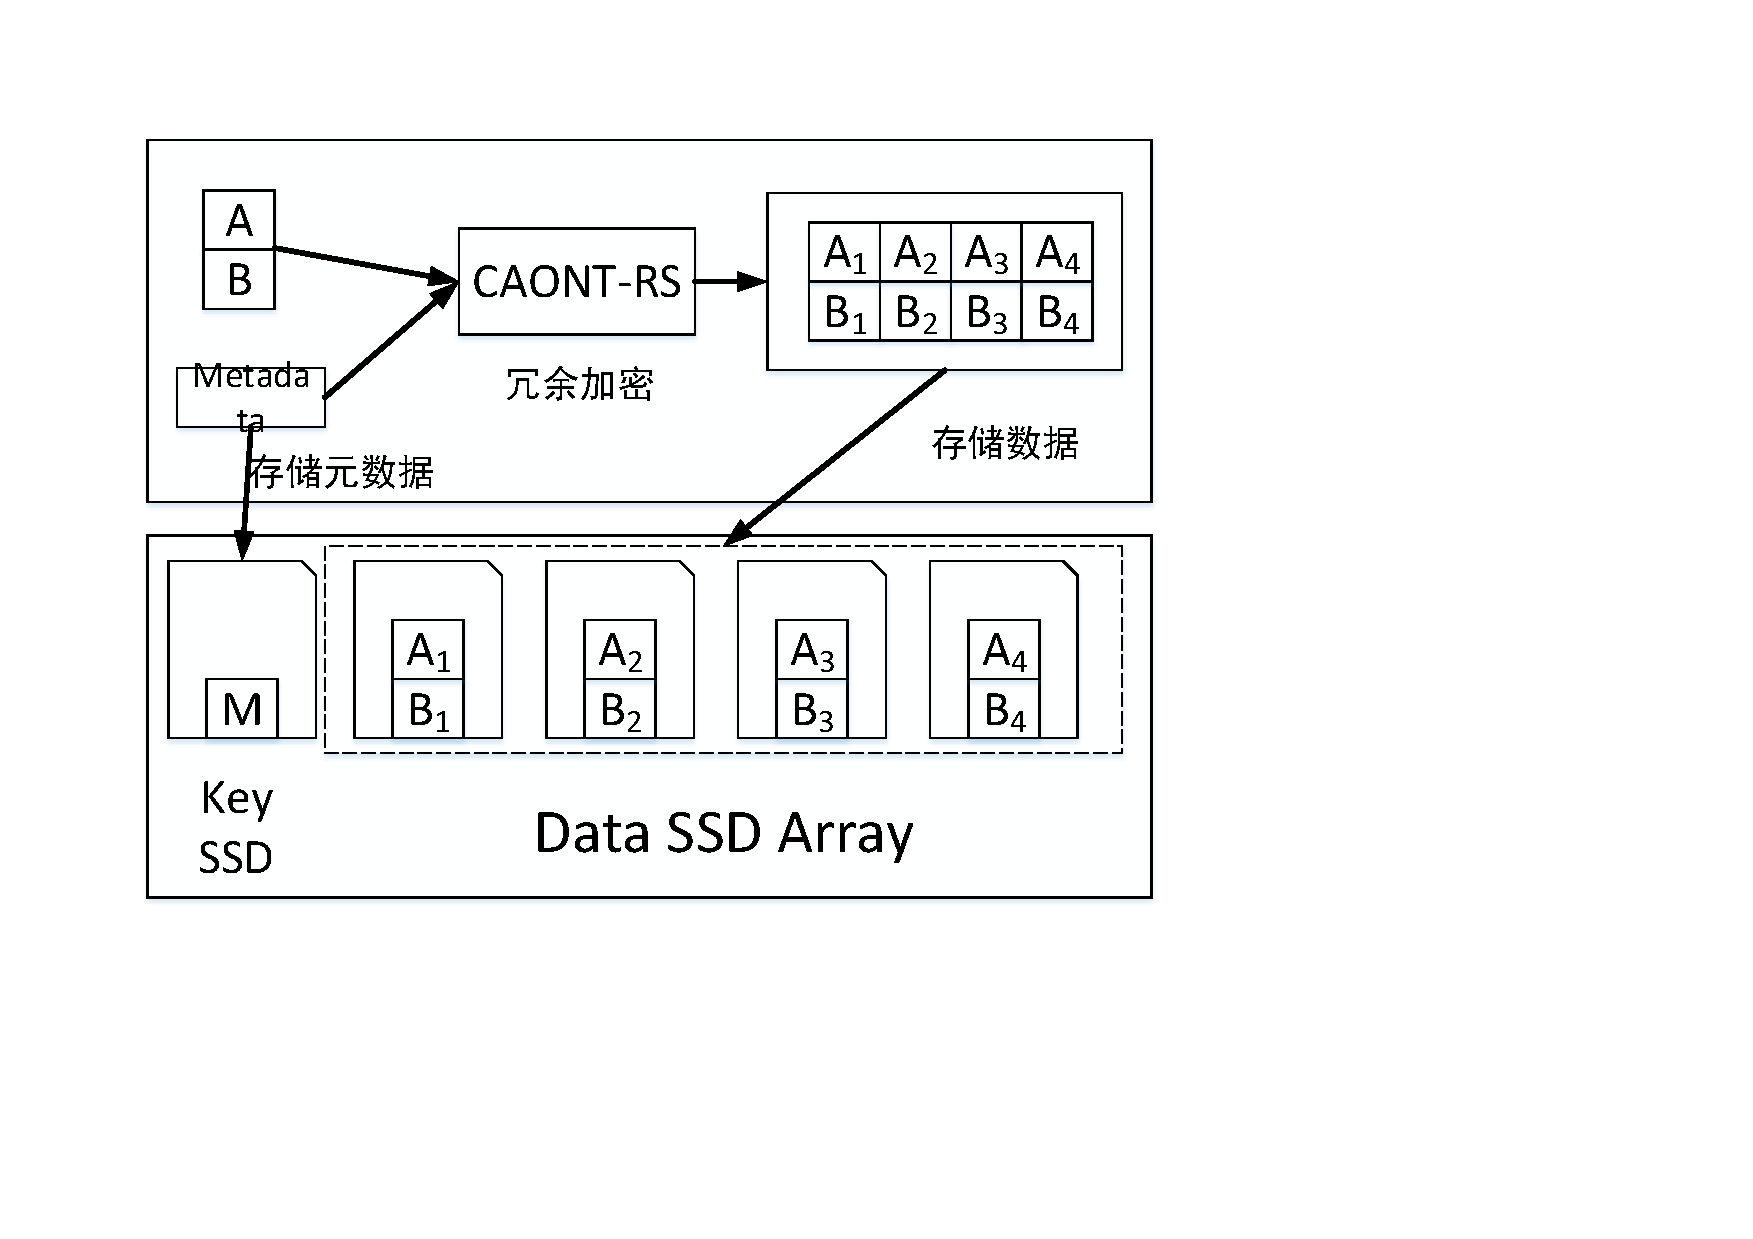
\includegraphics[width=4in]{Pics/data-write-st.pdf}
	\caption{数据写入架构}\label{fig:9}
\end{figure}
\begin{figure}[H]
	\centering
	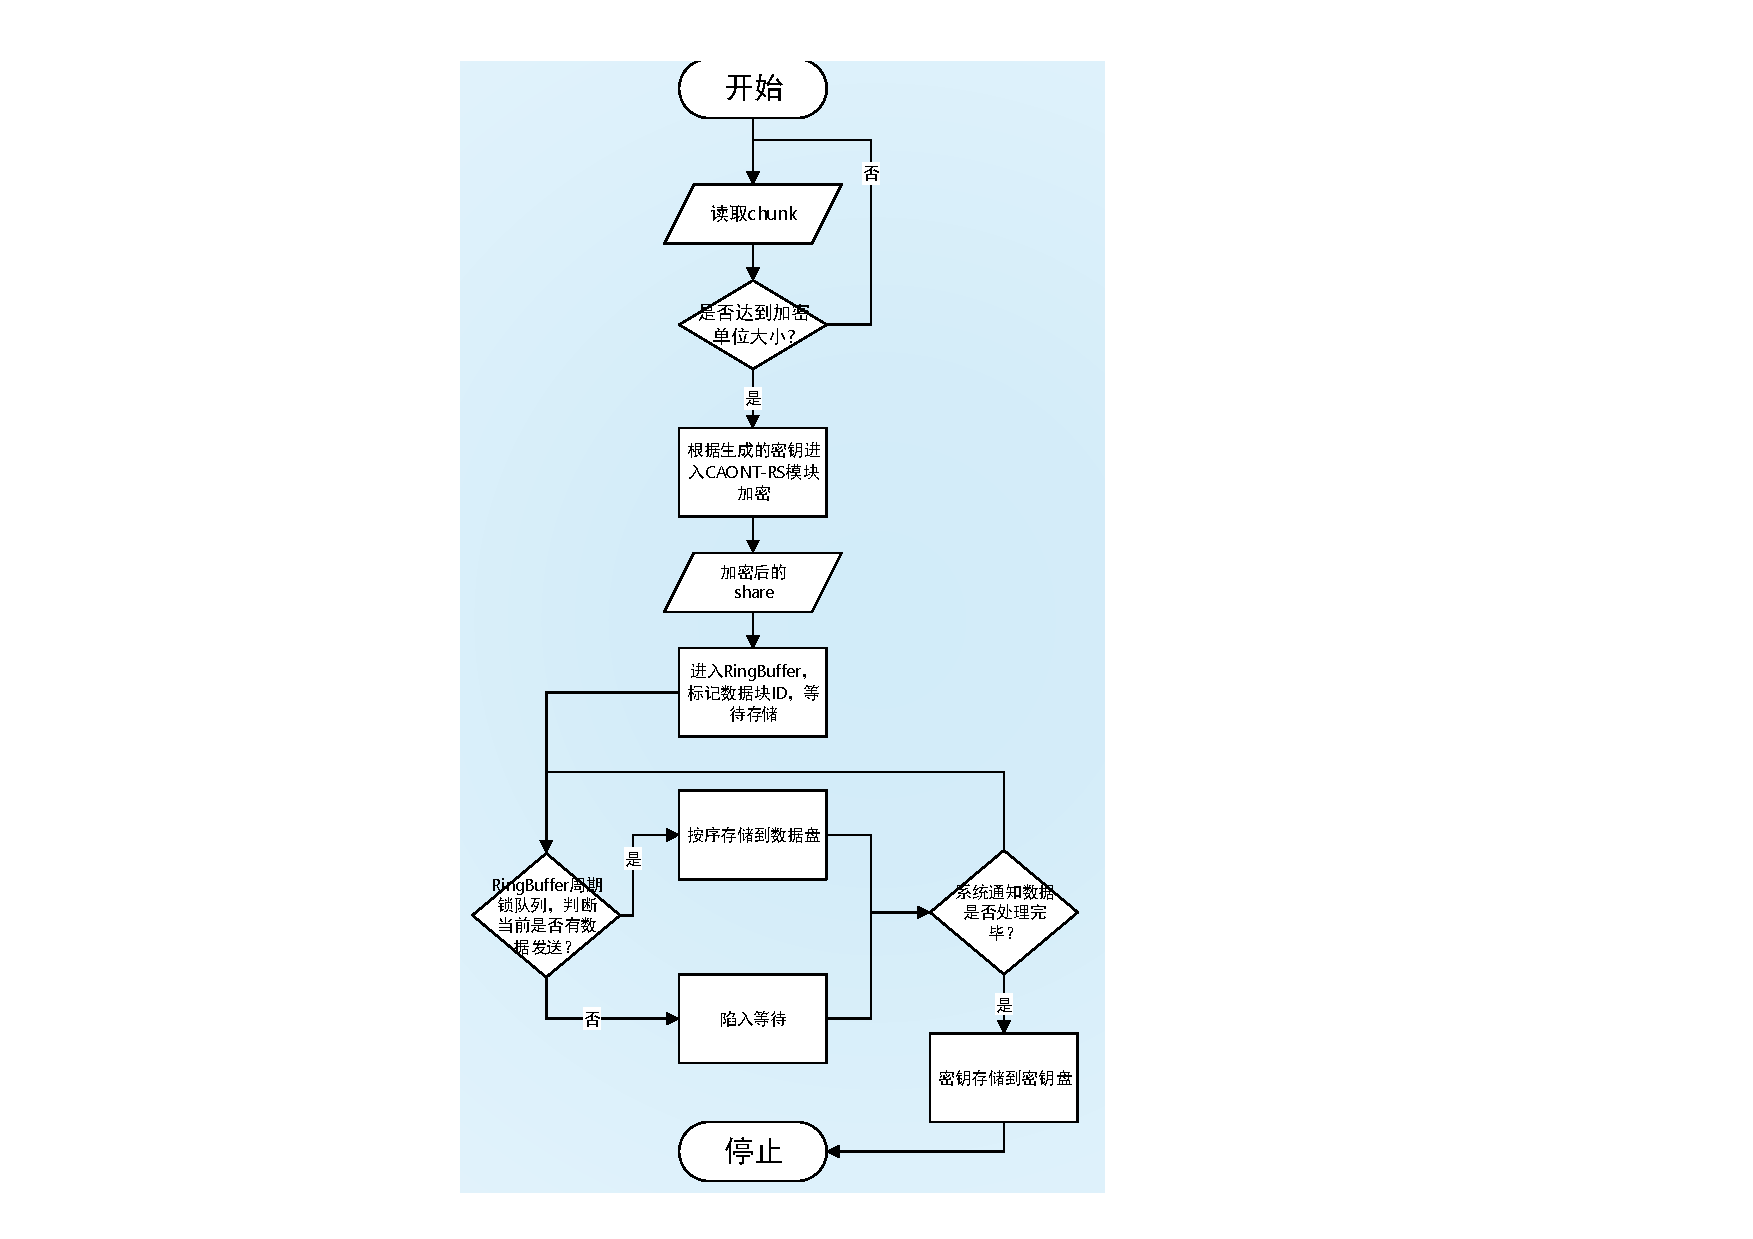
\includegraphics[width=4in]{Pics/data-write-pr.pdf}
	\caption{数据写入流程}\label{fig:10}
\end{figure}
在\autoref{fig:9}的数据写入存储结构以及\autoref{fig:10}数据写入流程中,当系统写入文件时,加密模块首先判断数据是否达到加密单元的大小,并且这个数据大小粒度可以调整。与此同时,密钥模块随机产生一段初始化数据,与原文件的元数据一起输入到加密模块,产生冗余的加密数据单元,并且按照顺序缓存到循环队列中等待存储,循环队列周期性地检查是否有数据需要转发存储,将数据依据数据盘的数量依次轮询发送存储请求。数据处理完毕,密钥模块将元数据存放到密钥盘,整个系统的加密写入流程完成。
\subsection{系统读取数据}
\begin{figure}[H]
	\centering
	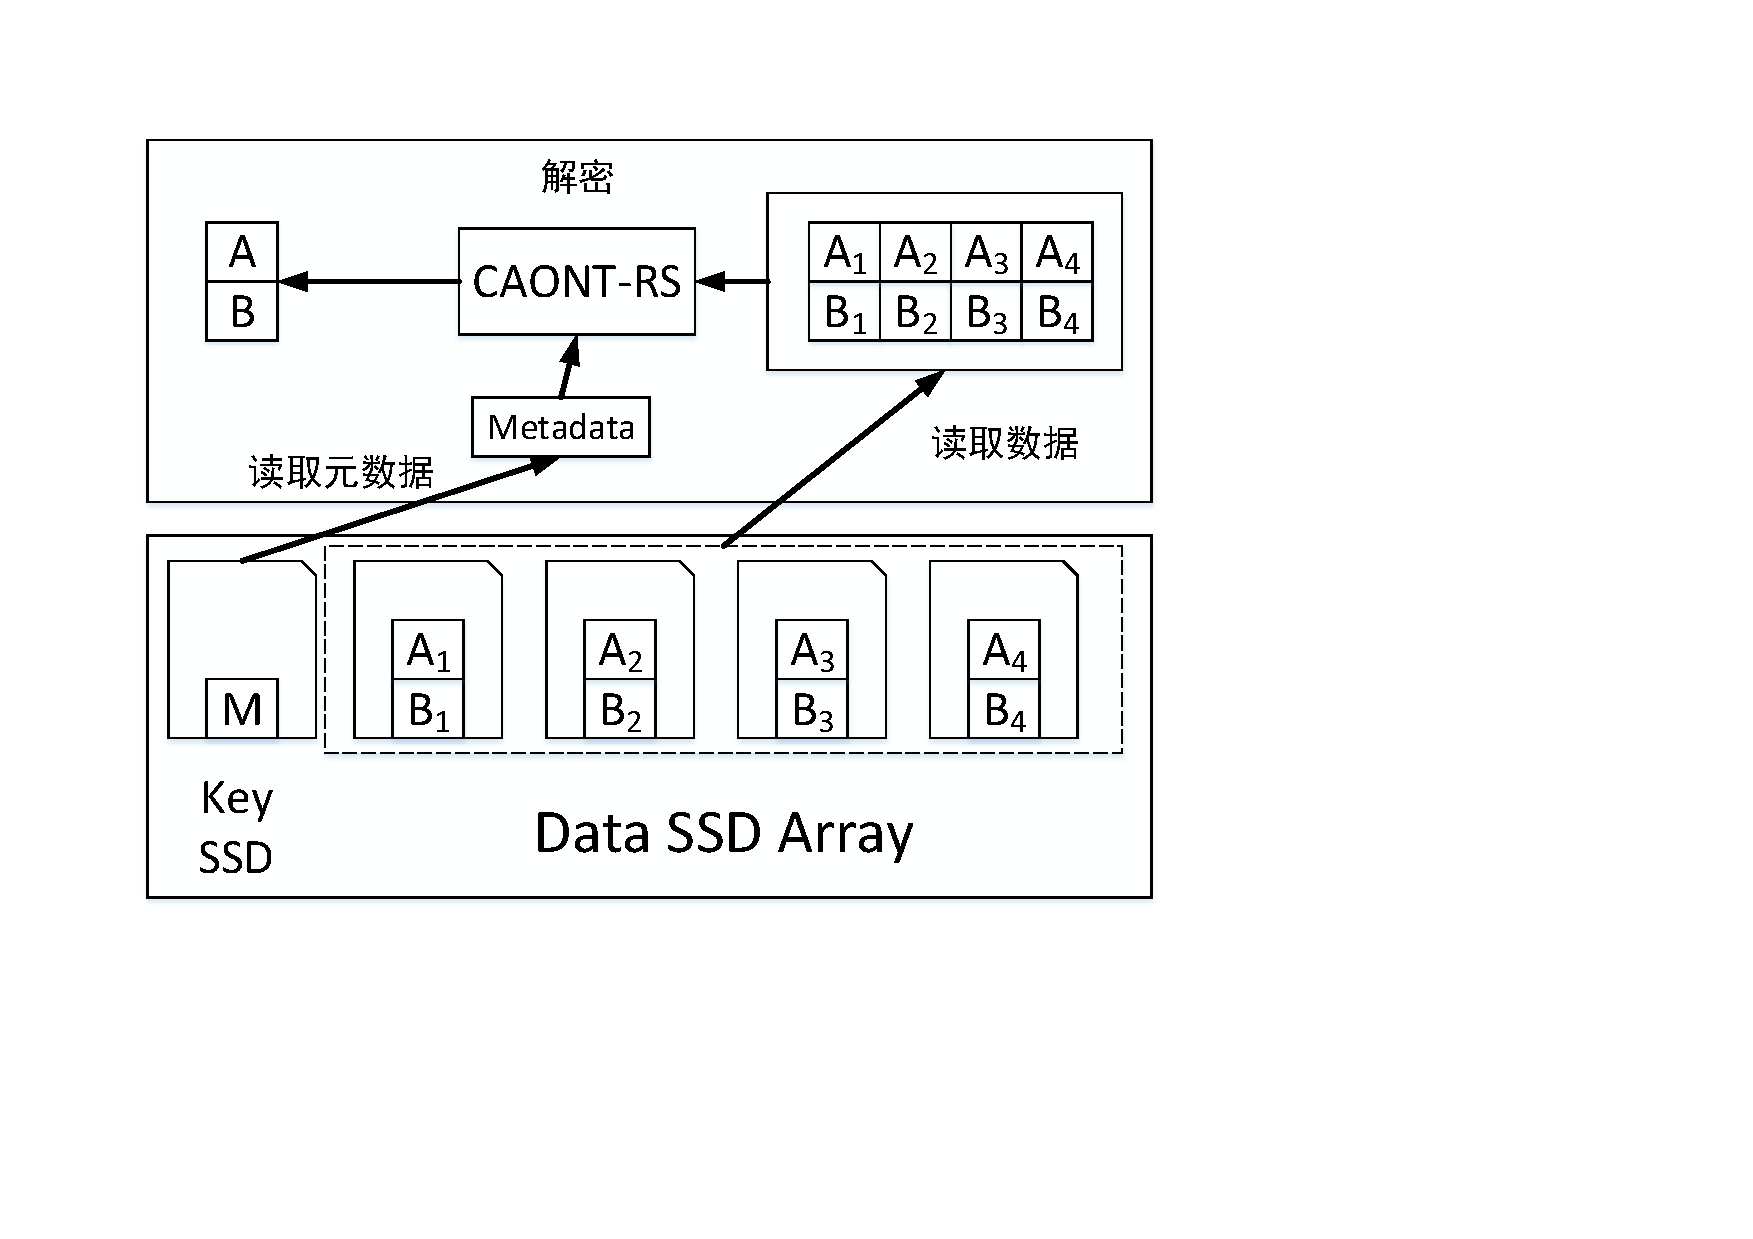
\includegraphics[width=4in]{Pics/data-read-st.pdf}
	\caption{数据读取架构}
    \label{fig:11}
\end{figure}
\begin{figure}[H]
	\centering
	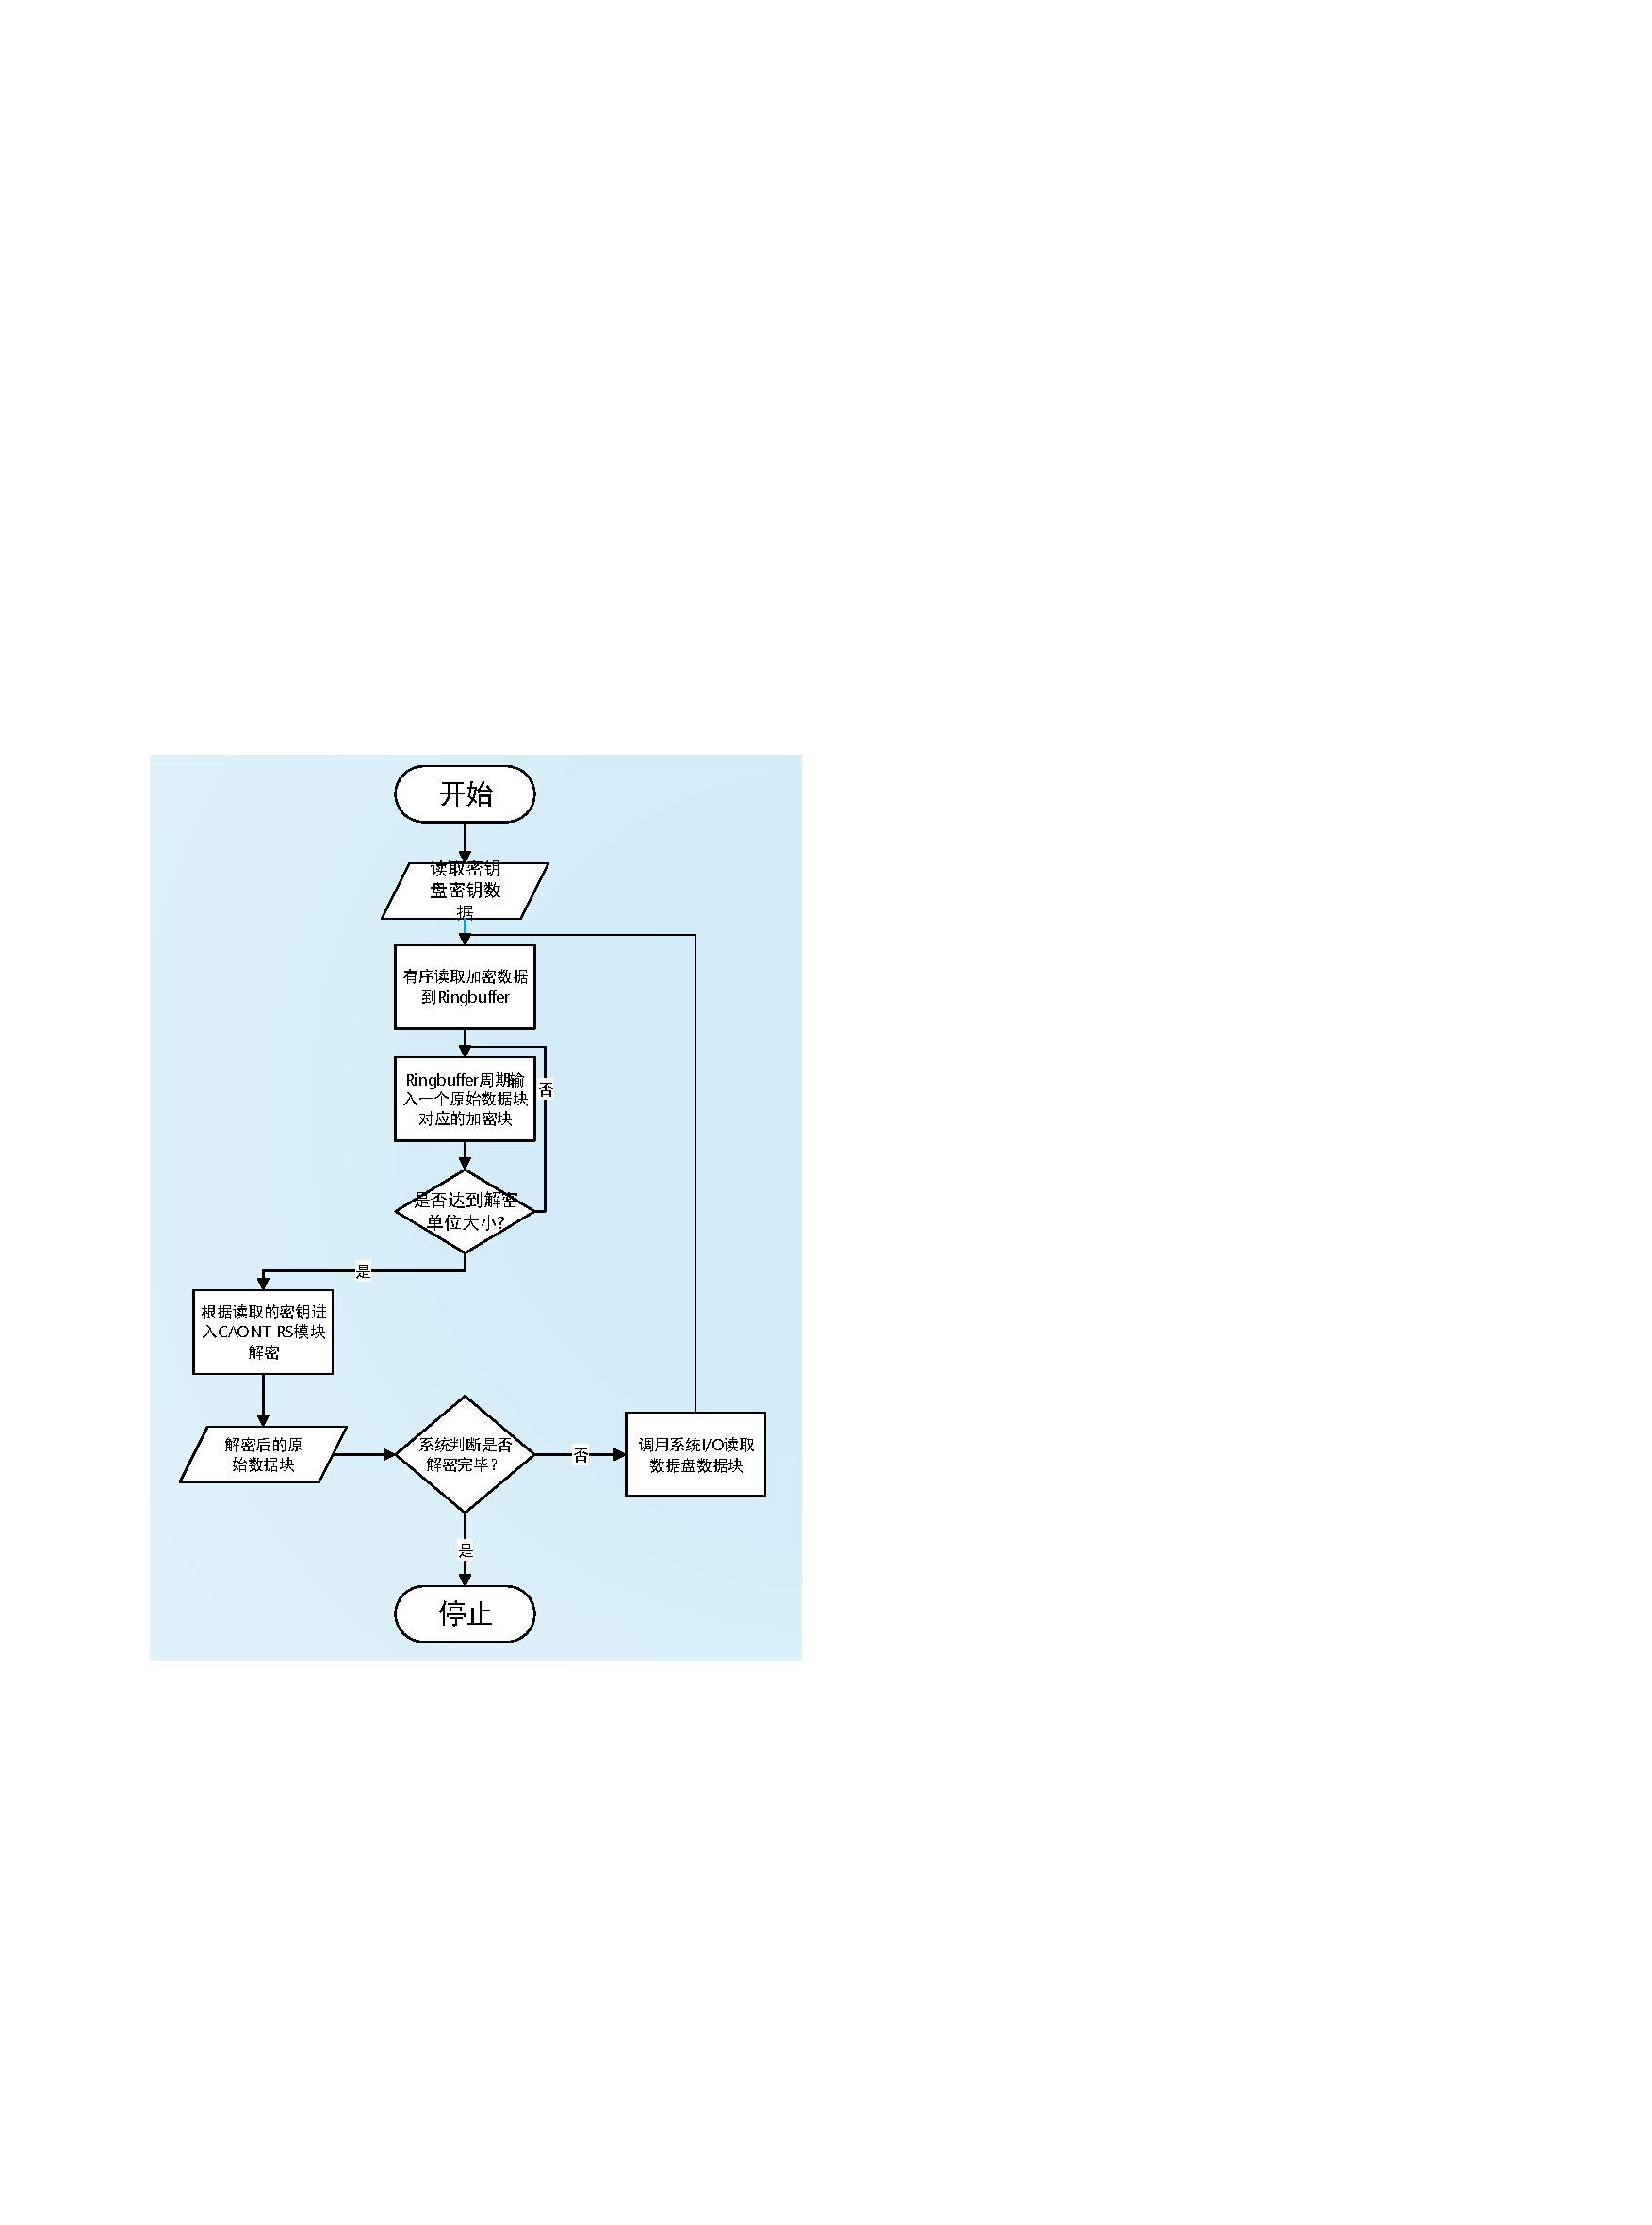
\includegraphics[width=4in]{Pics/data-read-pr.pdf}
	\caption{数据读取流程}
    \label{fig:12}
\end{figure}
在\autoref{fig:11}所示的数据读取结构和\autoref{fig:12}的数据读取流程中,当需要读取原始数据时,密钥模块首先读取密钥盘上的元数据,初始化密钥。然后数据分发模块按照次序读取各个数据盘上的加密单元数据,并缓存在循环队列里。当数据符合解密单元大小时,加密模块利用数据和密钥解密出原始数据块。系统处理完加密数据后,原始数据已被全部解密还原,数据读取流程结束。
\subsection{安全删除密钥数据}
由于每个单位大小的原始数据块的元数据很小,因此相比加密后的数据块来说,元数据的数据量很小,在密钥盘上存储的区域范围也很小,针对密钥盘的全盘擦除所花费的时间很少,而且,擦除数据时,真正有用的部分也只是针对这一块区域的数据进行覆写,从密钥盘的闪存使用寿命角度来说,这部分的擦除数据对于整体的固态盘擦除寿命影响很小。
\begin{figure}[H]
	\centering
	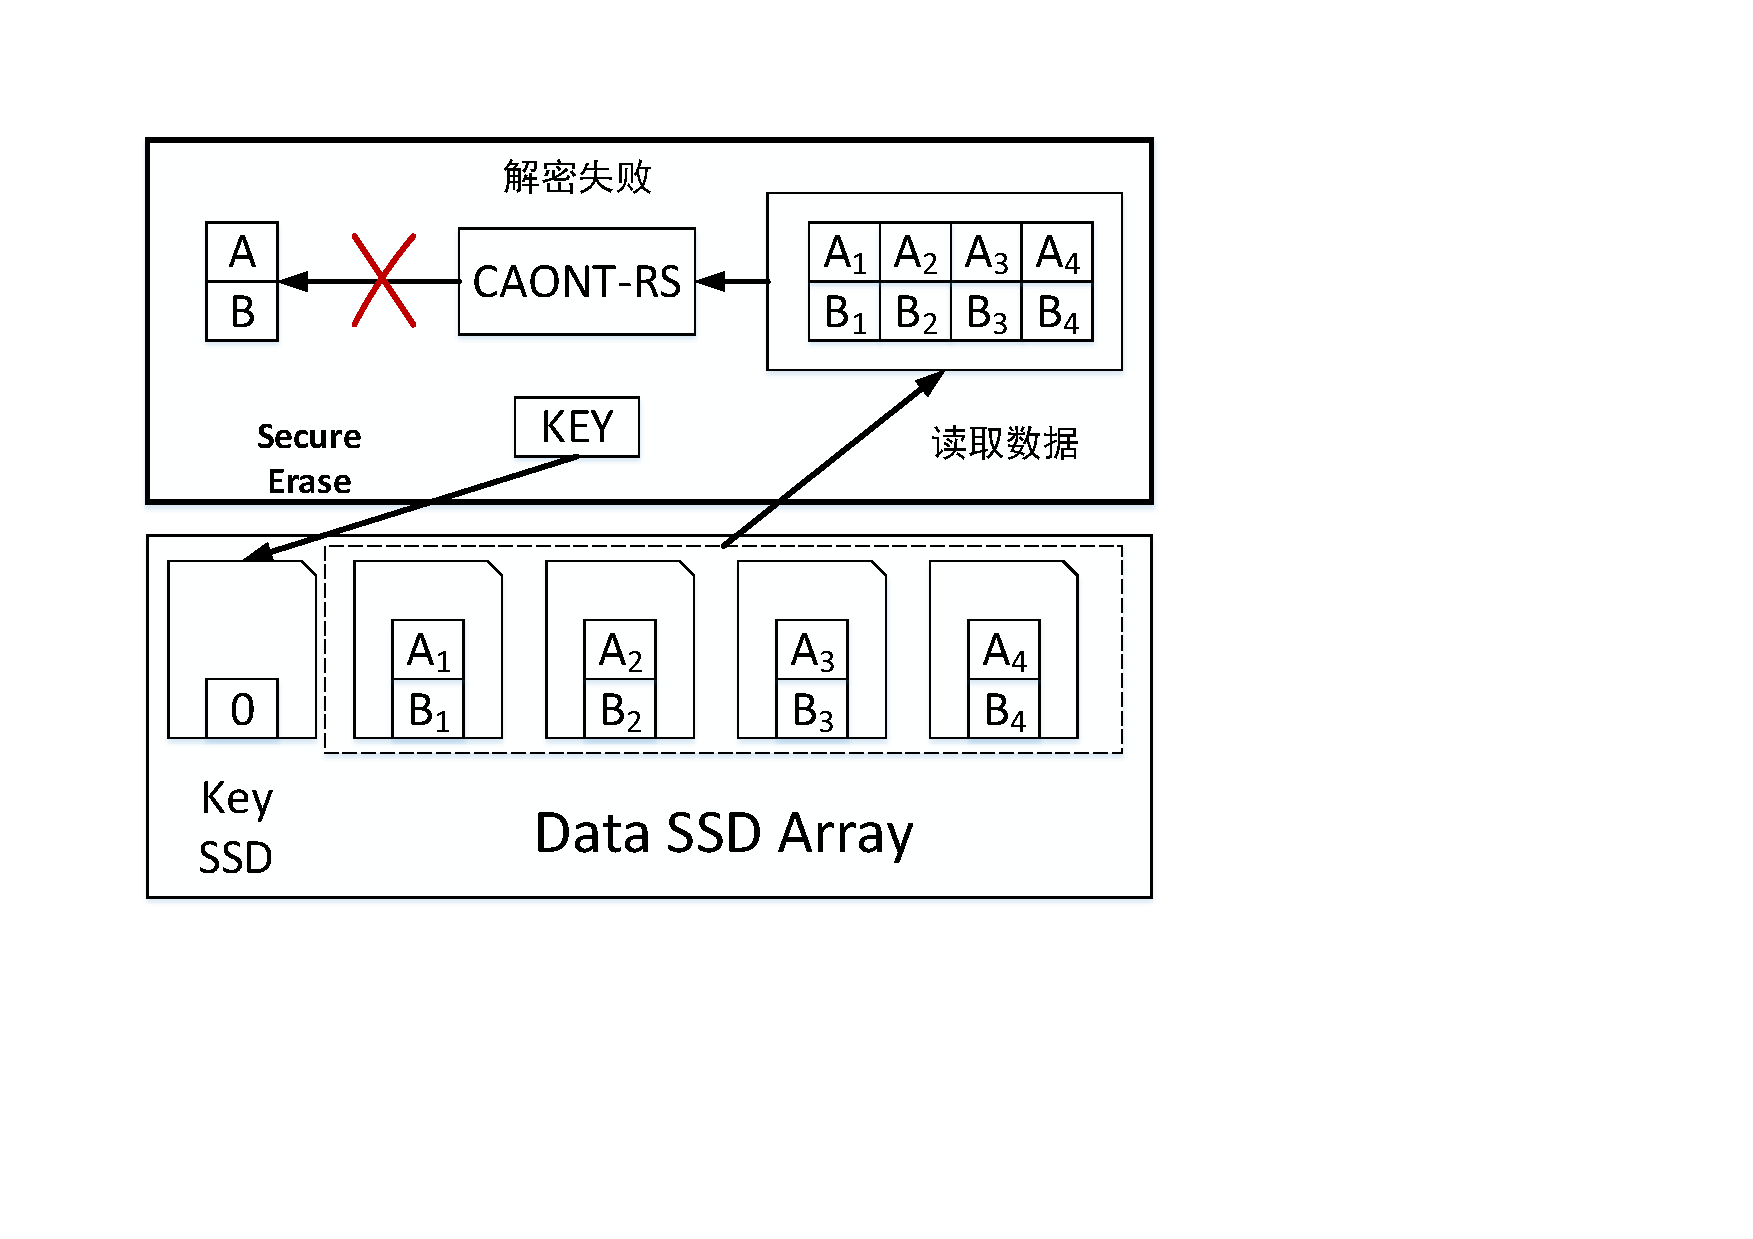
\includegraphics[width=4in]{Pics/del-key-st.pdf}
	\caption{擦除元数据进行安全验证架构}\label{fig:13}
\end{figure}
\begin{figure}[H]
	\centering
	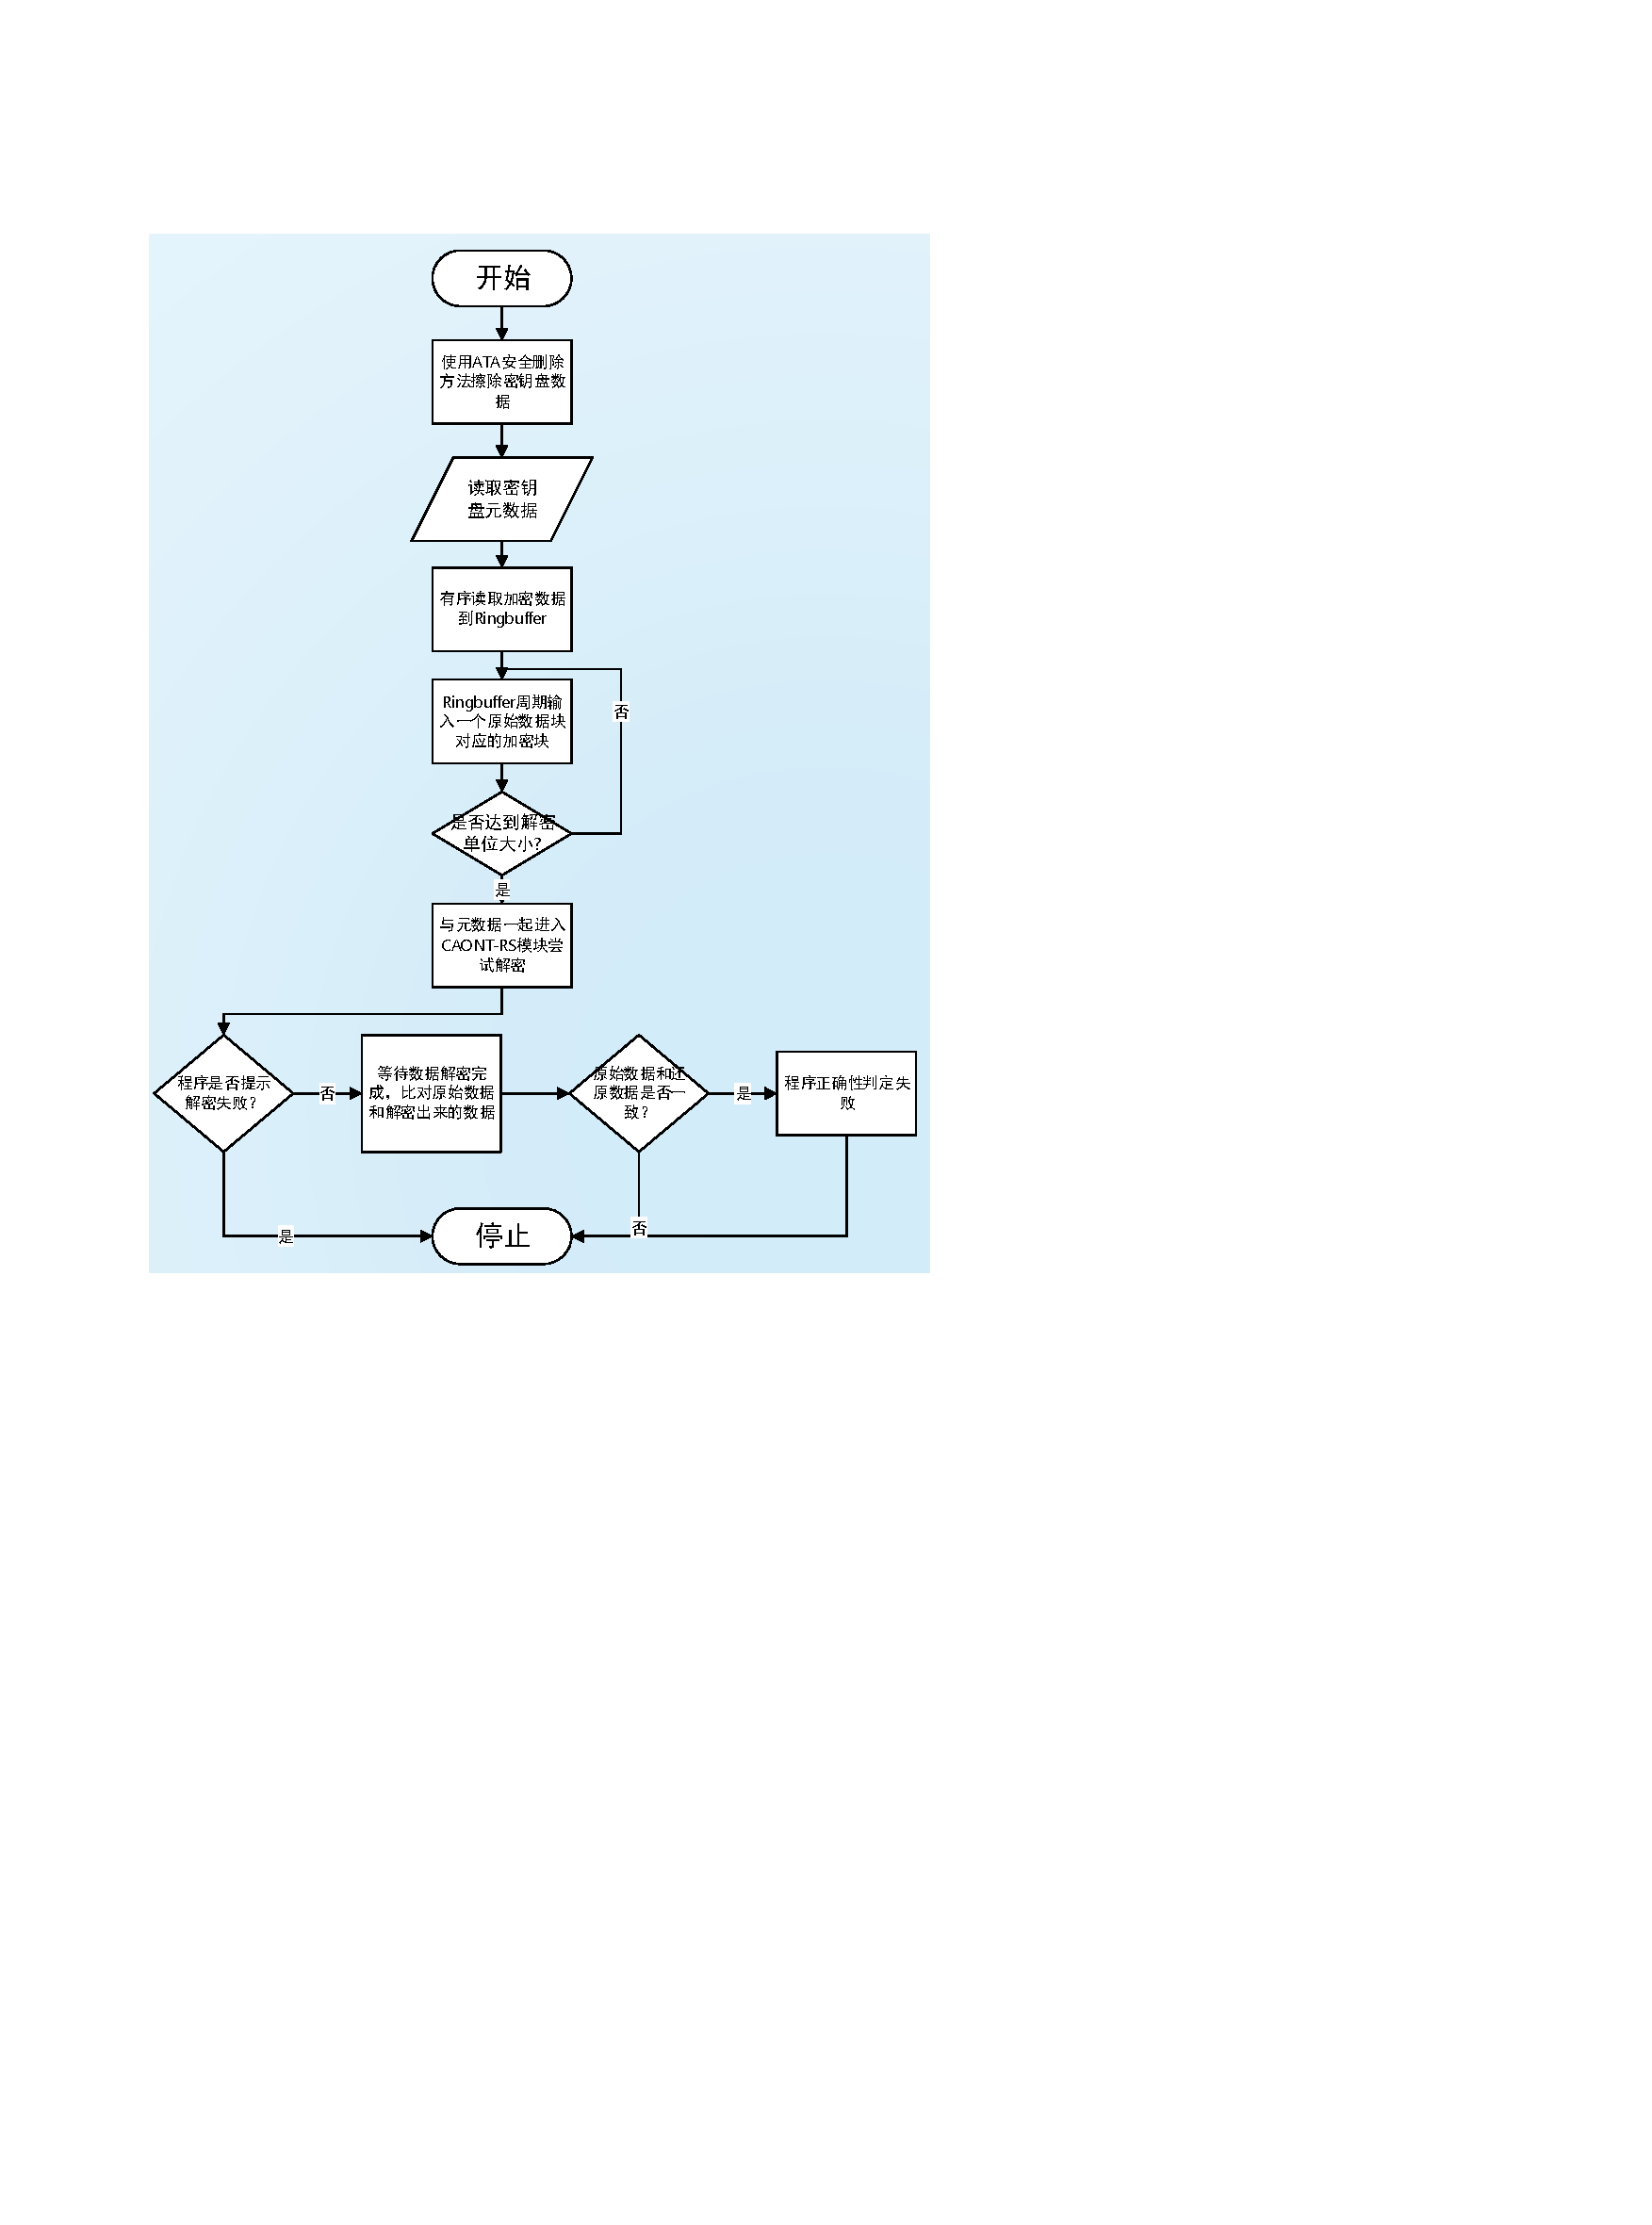
\includegraphics[width=4in]{Pics/del-key-pr.pdf}
	\caption{擦除元数据进行安全验证流程}\label{fig:14}
\end{figure}
在\autoref{fig:13}所示的删除元数据信息以及\autoref{fig:14}的删除后进行安全验证流程中,对密钥盘进行数据覆写时,使用了固态盘物理页覆写的技术。即美国加利福尼亚大学的研究人员通过实验证实\cite{Wei2011Reliably},目前市面上的 SLC 闪存基本都支持覆盖写入(只能将 1 改成 0),即可以在擦除前对物理页进行覆写(即第二次写操作),而对闪存的错误率并不产生明显的影响。
因此整个擦除手段如算法\autoref{alg:1}进行,在上层系统激活了删除功能时,系统立即调用密钥盘的TRIM命令对密钥盘无用数据标记无效,然后针对密钥盘采取多次全盘覆写操作,具体操作如\autoref{fig:14}所示的擦除实现:首先使用安全擦除工具擦除密钥盘上的全部数据,这种擦除手段是先向每一个物理页覆写数据0,然后再次向物理页覆写随机数据,最后覆写一次数据0,达到安全删除的目的。
\begin{algorithm}[H]
\caption{Secure Erase data Hash informathons.(Key data)}
\label{alg:1}
\begin{algorithmic}
	\REQUIRE
	$addr$: address of the NAND flash page;
	$i$: position of page
	$data$: page content
	\STATE {// 1. write zero to each page}
	\STATE $data \gets 0$
	\FOR{$i=0$ to SSD page total size}
	\STATE write data to page $addr_i$
	\ENDFOR
	\STATE // 2. write random bit to each page
	\FOR{$i=0$ to SSD page total size}
	\STATE write random bit to page $addr_i$
	\ENDFOR
	\STATE // 3. write zero to each page again.
	\STATE $data \gets 0$
	\FOR{$i=0$ to SSD page total size}
	\STATE write data to page $addr_i$;
	\ENDFOR
\end{algorithmic}
\end{algorithm}


此时密钥盘上的元数据已经被清除,然后密钥模块尝试读取元数据,同时数据分发模块获取每个数据盘上的加密数据,放入循环队列中缓存,加密模块尝试对数据进行解密操作,如果解密过程出现错误则说明元数据已经被更改,有效地阻止了数据被还原出来。如果解密流程正常进行,则比对最后被还原的数据和初始的数据内容,两者不一致则说明系统安全删除功能正常,否则判定失败。

\section{本章小结}
本文是全文的重点之一,旨在阐述全闪存盘阵的数据安全删除方案的设计,首先介绍了本方案依赖的前提和安全删除的技术关键,
然后按照本方案的各个模块定义介绍了数据加密方法,破坏数据恢复的条件以达到安全删除的目的,最后依次详细介绍了写入、读取、安全删除数据这些功能的架构和流程。
